\documentclass{article}
\title{Topologia Algébrica}
%\usepackage{import}
\usepackage{amsmath} %propósitos gerais
\usepackage{amssymb} % comandos como \mathbb
\usepackage{amsthm} % criar novos teoremas

\newif\ifplastex
\plastexfalse
\ifplastex
\else
\usepackage{mdframed} %criar caixas em volta de ambientes
\fi
%-----------------------------------------------------------------------------------------------!!!!Adicionar pacotes apenas acima dessa linha!!!!--------------------------------------------------------------------------------------------
\usepackage{hyperref} %referencias internas e externas


%novos estilos
\ifplastex

\else
\mdfdefinestyle{MyFrame}{%
	innertopmargin=\baselineskip,
	innerbottommargin=\baselineskip,
	innerrightmargin=20pt,
	innerleftmargin=20pt}
\fi

%novos ambientes e teoremas
\theoremstyle{definition}
\newtheorem{defi}{Definição}

\theoremstyle{plain}
\newtheorem{thm}{Teorema}
\newtheorem{prop}{Proposição}
\newtheorem{lemma}{Lema}
\newtheorem{af}{Afirmação}
\newtheorem{corol}{Corolário}
\newtheorem{ex}{Exemplo}

\theoremstyle{remark}
\newtheorem{nota}{Nota}
\ifplastex


\newenvironment{titlemize}[1]{%
	\textbf{{#1}}
	\begin{itemize}}
	{\end{itemize}}

\else

\newenvironment{titlemize}[1]{%
	\begin{mdframed}[style=MyFrame]
	\textbf{{#1}}
	\begin{itemize}}
	{\end{itemize} \end{mdframed}}

\fi
\newenvironment{dem}{
	\begin{proof}[{\bf Demonstração:}]}
	{\end{proof}}
%novos comandos

%comandos renovados



\begin{document}
\maketitle
%-------------------------------------------------------------------------------------------------------------!Draft!-------------------------------------------------------------------------------------------------------------------------
\section{Topologia quociente}
\label{topologia-quociente}
Um assunto que aparece de forma recorrente na topologia algébrica é o conceito de topologia quociente, que exploraremos a seguir. 

\subsection{Topologia Quociente}
\label{topologia-quociente-def}
\begin{titlemize}{Lista de dependências}
	\item \hyperref[topologia final]{Topologia Final}; 
\end{titlemize}
\begin{defi}[Topologia Quociente]
	Seja \(X\) um espaço topológico e \(\sim\) uma relação de equivalência em \(X\).
	Podemos conferir ao espaço \(X/\sim\) uma estrutura de espaço topologíco da seguinte maneira. Considere a função projeção
	\begin{align*}
		\pi:X&\to X/\sim;\\
		x&\mapsto [x].
	\end{align*}
	Podemos fazer com que \(\pi\) seja uma função contínua dando, para \(X/\sim\) a topologia final com relação à \(\pi\). Isto é, os abertos de \(X/\sim\) são exatamente imagens de abertos em \(X\) por \(\pi\).  
\end{defi}
Varios exemplos importantes de espaços topológicos com os quais trabalharemos no estudo de topologia algébrica podem ser construídos como espaços quocientes. Em particular uma construção muito útil é a de quocientar um espaço por um subespaço, como explicado na seguinte definição.
\begin{defi}[Quociente por um subespaço]
	Seja \(X\) um espaço topológico e \(A \subseteq X\) um subespaço. Definimos a seguinte relação binária, \(\sim_{A}\):\\
	\(a\sim b\) se e somente se \(a=b\) ou \(a,b\in A\). Essa relação é uma relação de equivalência, e assim define um espaço \(X/\sim_A\). Esse espaço será denotado por \(X/A\). 
\end{defi}
Um exemplo desse tipo de construção é a esfera \(S^1\) que pode ser construida como \(I/\{0,1\}\) onde \(I=[0,1]\). 
\begin{titlemize}{Lista de consequências}
	\item \hyperref[pinched-torus-ex]{Torus Pinçado};
\end{titlemize}


% onde conteudos.tex é o nome do arquivo tex que voce quer incluir nessa secção.
\subsection{Função contínua em topologia quociente}
\label{funcao-continua-em-topologia-quociente-prop}
\begin{titlemize}{Lista de dependências}
	\item \hyperref[topologia-quociente-def]{Topologia quociente}; 
\end{titlemize}

\begin{prop}
    Sejam $X,Y$ espaços topológicos. E seja $\sim$ uma relação de equivalência em $X$. Uma função $f:(X/\sim) \longrightarrow Y$ é contínua se e somente se $f\circ \pi$ é contínua, onde $\pi$ é a função projeção associada ao quociente.
\end{prop}
\begin{dem}
    Por um lado, suponhamos que $f$ seja contínua. Como a composição de funções contínuas é contínua, a função $f\circ \pi$ também seré contínua.

    Por outro lado, suponhamos que $f\circ \pi$ seja contínua. Seja $V\subseteq Y$ um aberto, pela hipóteses, $\pi^{-1}(f^{-1}(V))$ é um aberto. Agora, pela definição de topologia quociente, $f^{-1}(V)$ é um aberto em $X/\sim$, o que implica que $f$ é contínua. 
\end{dem}

Dois exemplos importantes de espaços quociente são os seguintes.
%-------------------------------------------------------------------------------------------------------------!Draft!-------------------------------------------------------------------------------------------------------------------------
\section{Cone e Suspensão sobre Espaços Topológicos}
\label{cone-suspensao}
%---------------------------------------------------------------------------------------------------------------------!Draft!-----------------------------------------------------------------------------------------------------------------
\subsection{Cone sobre um Espaço Topológico}
\label{cone-def}
\begin{titlemize}{Lista de dependências}
	\item \hyperref[topologia-quociente-def]{Topologia Quociente}.
\end{titlemize}

\begin{defi}[Cone]
    Dado um espaço topológico $X$, definimos o \textbf{cone sobre $X$} como o espaço quociente $X\times I/\sim$,
    onde $I=[0,1]$ é o intervalo com a topologia usual de subespaço de $\mathbb{R}$, e $\sim$ é a relação de equivalência tal que para todos $(x,s),(y,t) \in X\times I$,\\
    \centerline{
    $(x,s)\sim(y,t) \Leftrightarrow (x,s)=(y,t)$ ou $s=t=1$.}
\end{defi}

Tal construção é semelhante a de \hyperref[suspensao-def]{suspensão sobre um espaço topológico}.

\begin{titlemize}{Lista de consequências}
	%\item \hyperref[consequencia1]{Consequência 1};\\ %'consequencia1' é o label onde o conceito Consequência 1 aparece
	%\item \hyperref[]{}
    \item \hyperref[suspensao-cone-duplo-prop]{A construção de suspensão coincide com a de cone duplo}
\end{titlemize}
%---------------------------------------------------------------------------------------------------------------------!Draft!-----------------------------------------------------------------------------------------------------------------
\subsection{Suspensão sobre um Espaço Topológico}
\label{suspensao-def}
\begin{titlemize}{Lista de dependências}
	\item \hyperref[topologia-quociente-def]{Topologia Quociente}.
\end{titlemize}
\begin{defi}[Suspensão]
	Dado um espaço topológico $X$, definimos a \textbf{suspensão sobre X} como o espaço quociente $X\times [-1,1]/\sim$, onde $[-1,1]$ é munido da topologia usual de subespaço de $\mathbb{R}$, e $\sim$ é a relação de equivalência tal que para todos $(x,s),(y,t) \in X\times [-1,1]$,\\
    \centerline{
    $(x,s)\sim(y,t) \Leftrightarrow (x,s)=(y,t)$ ou $s=t=1$ ou $s=t=-1$.}
\end{defi}

Tal construção é semelhante a de \hyperref[cone-def]{cone sobre um espaço topológico}.

\begin{titlemize}{Lista de consequências}
	%\item \hyperref[consequencia1]{Consequência 1};\\ %'consequencia1' é o label onde o conceito Consequência 1 aparece
	\item \hyperref[suspensao-cone-duplo-prop]{A construção de suspensão coincide com a de cone duplo}
\end{titlemize}
Seguem alguns resultados relevantes sobre cones e suspensões:
%---------------------------------------------------------------------------------------------------------------------!Draft!-----------------------------------------------------------------------------------------------------------------
\subsection{Suspensão coincide com Cone Duplo}
\label{suspensao-cone-duplo-prop}
\begin{titlemize}{Lista de dependências}
	\item \hyperref[cone-def]{Cone};\\
	\item \hyperref[suspensao-def]{Suspensão}.
\end{titlemize}
Provaremos que a suspensão sobre um espaço topológico é homeomorfa a um cone duplo, confirmando as intuições sobre os objetos.
\begin{prop}[A construção de suspensão coincide com a de cone duplo]
	Dado $X$ um espaço topológico, considere os espaços
    \[S(X) = X\times[-1,1]/\sim_S\hspace{6 pt} = \{[x,t]_S : x\in X, t\in [-1,1]\},\]
    \[C(X) = X\times I/\sim_C\hspace{6 pt} = \{[x,t]_C : x\in X, t\in I\}.\]
    \\
    \noindent E sobre $C(X) \amalg C(X) = C(X)\times\{-1,1\}$, seja $\sim$ a relação de equivalência\\
    \\ \centerline{
    $([x,s]_C,i) \sim ([y,t]_C,j) \Leftrightarrow ([x,s]_C,i) = ([y,t]_C,j)$ ou $(x=y$ e $s=t=0)$}\\
    \\para todos $x,y \in X$, $s,t \in I$ e $i,j \in \{-1,1\}$.    
    
    Defina a função \begin{align*}
        \psi: S(X) &\rightarrow (C(X) \amalg C(X))/ \sim\\
                [x,t]_S &\mapsto [[x,|t|]_C,\text{sgn}(t)]
    \end{align*}
    onde $\text{sgn}(t) = -1$ caso $t < 0$ e $\text{sgn}(t) = 1$ caso contrário. Então $\psi$ é homeomorfismo.

	Ou seja, a construção de suspensão sobre um espaço topológico coincide com a colagem de dois cones sobre o mesmo espaço topológico, quando identificamos as suas respectivas bases.

    \begin{dem}
        Primeiramente, $\psi$ está bem definida. Dado $(x,t) \in X\times I$, vale que $[x,t]_S = \{(x,t)\}$, se $t \in \left]-1,1\right[$, ou então $[(x,t)] = X\times\{t\}$, se $t \in \{-1,1\}$. Mas para quaisquer $x,x'\in X$ e $t\in \{-1,1\}$,\[
        [[x,|t|]_C,\text{sgn}(t)] =
        [X\times\{|t|\},\text{sgn}(t)] =
        [[x',|t|]_C,\text{sgn}(t)]
        \]
        e então está bem definido $\psi([x,t]_S)$.

        Denotemos por $\pi_S$, $\pi_C$ e $\pi$ as aplicações quociente canônicas com respeito a $\sim_S$, $\sim_C$ e $\sim$, respectivamente. Por \textbf{(adicionar proposição aqui)}, $\psi$ é contínua se, e somente se,\begin{align*}
            \psi \circ \pi_S: X\times[-1,1] &\rightarrow (C(X) \amalg C(X))/ \sim\\
            (x,t) &\mapsto [[x,|t|]_C,\text{sgn}(t)]
        \end{align*}
        for contínua. Para todo subconjunto aberto $U \subset C(X)\amalg C(X)/\sim\hspace{3pt}$, existem abertos $V,W \subset C(X)$ tais que $\pi^{-1}(U) = V\amalg W = (V\times\{-1\}) \cup (W\times\{1\})$. Por sua vez, $\pi_C^{-1}(V)$ e $\pi_C^{-1}(W)$ são abertos de $X\times[0,1]$. Então,
        \begin{align*}
        (\psi \circ \pi_S)^{-1}(U)
        &= (\psi \circ \pi_S)^{-1}(\pi(V\times\{-1\}) \cup \pi(W\times\{1\}))\\
        &= (\psi \circ \pi_S)^{-1}(\pi(V\times\{-1\})) \cup (\psi \circ \pi_S)^{-1}(\pi(W\times\{1\})).   
        \end{align*}
        
        Calculemos cada termo da união separadamente.
        \begin{align*}
            (\psi \circ \pi_S)^{-1}(\pi(V\times\{-1\}))
            &= \{(x,t): [x,|t|]_C \in V, t \in [-1,0]\}\\
            &= \{(x,-t): [x,t]_C \in V, t \in I\}\\
            &= A(\pi_C^{-1}(V))   
        \end{align*}
        onde $A: (x,t) \mapsto (x,-t)$. E analogamente, $(\psi \circ \pi_S)^{-1}(\pi(W\times\{1\})) = \pi_C^{-1}(W)$. Concluímos assim que
        \[(\psi \circ \pi_S)^{-1}(U) = A(\pi_C^{-1}(V)) \cup \pi_C^{-1}(W)\]
        é aberto, e então $\psi$ é contínua.
    \end{dem}
\end{prop}


\begin{titlemize}{Lista de consequências}
	%\item \hyperref[consequencia1]{Consequência 1};\\ %'consequencia1' é o label onde o conceito Consequência 1 aparece
	%\item \hyperref[]{}
    \item \hyperref[suspensao-euclidiano-prop]{Suspensão sobre subespaços de $\mathbb{R}^n$}
    \item \hyperref[suspensao-esfera-prop]{Suspensão sobre esferas $S^n\subset\mathbb{R}^{n+1}$}
\end{titlemize}


%---------------------------------------------------------------------------------------------------------------------!Draft!-----------------------------------------------------------------------------------------------------------------
\subsection{Cone sobre subespaços de $\mathbb{R}^n$}
\label{cone-euclidiano-prop}
\begin{titlemize}{Lista de dependências}
	\item \hyperref[cone-def]{Cone sobre um Espaço Topológico}.
\end{titlemize}
Provaremos que a construção de cone sobre um subespaço topológico de $\mathbb{R}^n$ (com a topologia usual) é homeomorfa à construção geométrica em $\mathbb{R}^{n+1}$, sendo assim uma generalização de conceitos que antes só faziam sentido no contexto de espaços euclidianos.
\begin{thm}[A construção de cone generaliza a de subespaços euclidianos]
	Seja $X \subset \mathbb{R}^n$. Então,\begin{align*}
        \phi: C(X) &\rightarrow \{((1-t) x_1,...,(1-t) x_n,t): (x_1,...,x_n) \in X, t \in [0,1]\}\subset \mathbb{R}^{n+1}\\
        [(x,t)] \mapsto ((1-t) x_1,...,(1-t) x_n,t), \forall x=(x_1,...,x_n)\in X, \forall t \in [0,1]
    \end{align*}
    é um homeomorfismo.\\
    Ou seja, para subespaços de $\mathbb{R}^n$, a construção de cone recupera a intuição geométrica e coincide enquanto espaço topológico com $\{((1-t)x,t):x\in X, t\in I\} \in \mathbb{R}^{n+1}$, onde $(x,t)$ denota concatenação de vetores.
\end{thm}

Tal proposição é análoga à sobre \hyperref[suspensao-euclidiano-prop]{suspensão sobre um espaço euclidiano}.

\begin{titlemize}{Lista de consequências}
	%\item \hyperref[consequencia1]{Consequência 1}.
	%\item \hyperref[]{}
\end{titlemize}
%---------------------------------------------------------------------------------------------------------------------!Draft!-----------------------------------------------------------------------------------------------------------------
\subsection{Suspensão sobre subespaços de $\mathbb{R}^n$}
\label{suspensao-euclidiano-prop}
\begin{titlemize}{Lista de dependências}
	\item \hyperref[suspensao-def]{Suspensão sobre um Espaço Topológico};
    \item \hyperref[suspensao-cone-duplo-prop]{Suspensão e Cone Duplo}
    \item \hyperref[cone-euclidiano-prop]{Cone sobre subespaços de $\mathbb{R}^n$}
\end{titlemize}
Provaremos que a construção de uma suspensão sobre um subespaço topológico de $\mathbb{R}^n$ (com a topologia usual) é homeomorfa à construção geométrica em $\mathbb{R}^{n+1}$, sendo assim uma generalização de conceitos que antes só faziam sentido no contexto de espaços euclidianos.

Nesse momento, dados $(x_1,x_2,...,x_n) \in \mathbb{R}^n$ e $t \in \mathbb{R}$, denotemos por $(x,t)$ o vetor $(x_1,x_2,...,x_n,t) \in \mathbb{R}^{n+1}$.

\begin{prop}[A construção de suspensão generaliza a de subespaços euclidianos]
	Seja $X \subset \mathbb{R}^n$, e considere\\
    \centerline{$S_g(X) = \{((1-|t|)x,t):x\in X, t\in [-1,1]\} \subset \mathbb{R}^{n+1}$.}\\
    Então,\begin{align*}
        \varphi: S(X) &\rightarrow S_g(X)\\
        [(x,t)] &\mapsto ((1-t)x,t), \forall x\in X, \forall t \in [-1,1]
    \end{align*}
    é um homeomorfismo.\\
    Ou seja, para subespaços de $\mathbb{R}^n$, a construção de suspensão recupera a intuição geométrica e coincide enquanto espaço topológico com $S_g(X)$.
\end{prop}

Tal proposição é análoga à sobre \hyperref[cone-euclidiano-prop]{cone sobre um espaço euclidiano}.

%\begin{titlemize}{Lista de consequências}
	%\item \hyperref[consequencia1]{Consequência 1};\\ %'consequencia1' é o label onde o conceito Consequência 1 aparece
	%\item \hyperref[]{}
%\end{titlemize}

%---------------------------------------------------------------------------------------------------------------------!Draft!-----------------------------------------------------------------------------------------------------------------
\subsection{Cone sobre esferas $S^n\subset\mathbb{R}^{n+1}$}
\label{cone-esfera-prop}
\begin{titlemize}{Lista de dependências}
	\item \hyperref[cone-def]{Cone sobre um Espaço Topológico}.
    %Definição de esfera e disco
\end{titlemize}

Nesse momento, dados $(x_1,x_2,...,x_n) \in \mathbb{R}^n$ e $t \in \mathbb{R}$, denotemos por $(x,t)$ o vetor $(x_1,x_2,...,x_n,t) \in \mathbb{R}^{n+1}$.

\begin{prop}[Cone sobre esferas]
	$C(S^n) \cong D^{n+1}$, para todo $n\geq 1$.
 
    \begin{dem}
        Pela \hyperref[cone-euclidiano-prop]{Proposição acerca de cones sobre subconjuntos de $\mathbb{R}^n$}, basta provar que $D^{n+1}\cong C_g(S^n) = \{((1-t)x,t):x\in S^n, t\in I\}$.

        Seja $\pi:\mathbb{R}^{n+1}\to\mathbb{R}^n$ a projeção dada por $\pi(x,t) = x$ para cada $(x,t) \in \mathbb{R}^{n+1}$.
        
        Defina $f:D^{n+1}\to C_g(S^n)$ como $f(p) = (p,1-\|p\|)$. $f$ está bem definida, pois $(p,1-\|p\|)=((1-t)x,t)$ para $t=1-\|p\|$, e $x=p/\|p\|$ caso $\|p\|\neq 0$ ou então $x\in S^n$ qualquer caso contrário. Tal raciocínio também mostra que $f$ é sobrejetora. $f$ é injetora, uma vez que $\pi \circ f(p) = p$.

        É fácil ver que $f$ é contínua.  Pelo Teorema de Heine-Borel, $D^{n+1} \subset \mathbb{R}^{n+1}$ é compacto, assim $f(D^{n+1})=C_g(S^n)$ também é. E ambos são Hausdorff, portanto $f$ é homeomorfismo e concluímos. 
    \end{dem}
\end{prop}

Tal proposição é análoga à sobre \hyperref[suspensao-esfera-prop]{suspensão sobre esferas}.

\begin{titlemize}{Lista de consequências}
	%\item \hyperref[consequencia1]{Consequência 1}.
	%\item \hyperref[]{}
\end{titlemize}
%---------------------------------------------------------------------------------------------------------------------!Draft!-----------------------------------------------------------------------------------------------------------------
\subsection{Suspensão sobre esferas $S^n\subset\mathbb{R}^{n+1}$}
\label{suspensao-esfera-prop}
\begin{titlemize}{Lista de dependências}
	\item \hyperref[suspensao-def]{Suspensão sobre um Espaço Topológico}
    \item \hyperref[suspensao-cone-duplo-prop]{Suspensão coincide com Cone Duplo}
    \item \hyperref[cone-esfera-prop]{Cone sobre esferas $S^n\subset\mathbb{R}^{n+1}$}
    %Definição de esfera e disco
\end{titlemize}

%Nesse momento, dados $(x_1,x_2,...,x_n) \in \mathbb{R}^n$ e $t \in \mathbb{R}$, denotemos por $(x,t)$ o vetor $(x_1,x_2,...,x_n,t) \in \mathbb{R}^{n+1}$.

Tal proposição é análoga à sobre \hyperref[cone-esfera-prop]{cone sobre esferas} e poderia ser provada de maneira análoga, porém a utilizaremos para facilitar a demonstração.

\begin{prop}[Suspensão sobre esferas]
	$S(S^n) \cong S^{n+1}$, para todo $n\geq 1$.

    \begin{dem}
        Pela \hyperref[suspensao-cone-duplo-prop]{caracterização de suspensão como cone duplo}, \[S(S^n) \cong (C(S^n) \amalg C(S^n))/\sim_0,\] onde $\sim_0$ identifica as bases dos cones. Já pela \hyperref[cone-esfera-prop]{Proposição acerca de cones sobre esferas}, $C(S^n) \cong D^{n+1}$, logo \[S(S^n) \cong (D^{n+1} \amalg D^{n+1})/\sim\] onde $\sim$ identifica os subconjuntos $S^n$ contidos em cada $D^{n+1}$.
        
        Basta então provar que o disco $D^{n+1}$ é homeomorfo a um hemisfério $H^{n+1} = S^{n+1}\cap (\mathbb{R}^n \times [0,\infty[)$. Seja $\pi:\mathbb{R}^{n+1}\to\mathbb{R}^n$ a projeção dada por $\pi(x,t) = x$ para cada $(x,t) \in \mathbb{R}^{n+1}$.
        
        De fato, $h:D^{n+1}\to H^{n+1}$ dada por $h(p)=(p,\sqrt{1-\|p\|^2})$ está bem definida, é contínua e é injetora pois $\pi \circ h(p) = p$. Por fim, é sobrejetora pois para todo ponto $(p,t)\in H^{n+1}$ vale que $t=\sqrt{1-\|p\|^2}$. Portanto, pelo mesmo argumento que na \hyperref[cone-esfera-prop]{Proposição acerca de cones sobre esferas}, concluímos que $h$ é homeomorfismo e então\[S(S^n) \cong (H^{n+1} \amalg H^{n+1})/\sim \hspace{6 pt} \cong S^{n+1}.\]
    \end{dem}
\end{prop}

%\begin{titlemize}{Lista de consequências}
	%\item \hyperref[consequencia1]{Consequência 1}.
	%\item \hyperref[]{}
%\end{titlemize}


%%% Local Variables:
%%% mode: LaTeX
%%% TeX-master: "../Alg.Top-Wiki"
%%% End:

%---------------------------------------------------------------------------------------------------------------------!Draft!-----------------------------------------------------------------------------------------------------------------
\subsection{Espaços Quociente e a propriedade Hausdorff} %afirmação aqui significa teorema/proposição/colorário/lema
\label{topologia-quociente-hausdorff-thm}
\begin{titlemize}{Lista de dependências}
	\item \hyperref[topologia-quociente-def]{Espaços Quociente};\\ %'dependencia1' é o label onde o conceito Dependência 1 aparece (--à arrumar um padrão para referencias e labels--) 
% quantas dependências forem necessárias.
\end{titlemize}
Comentário sobre os objetos envolvidos na afirmação.
\begin{thm}[Espaços quocientes Hausdorff]% ou af(afirmação)/prop(proposição)/corol(corolário)/lemma(lema)/outros ambientes devem ser definidos no preambulo de Alg.Top-Wiki.tex 
Sejam $X$ um espaço Hausdorff e $\sim$ uma relação de equivalência em $X$ para a qual a projeção $\pi: X \rightarrow X/\sim$ é uma aplicação aberta. Defina o conjunto $R=\{(x,x')\in X\times X| x\sim x'\}$.

Então $X/\sim$ é Hausdorff se, e somente se, $R\subset X\times X$ é fechado.

\end{thm}
\begin{dem}
    $(\Longrightarrow)$ Se $X/\sim$ é de Hausdorff, gostaríamos de mostrar que $X\times X\backslash R$ é aberto. Para qualquer ponto $(x,x')\in (X\times X)\backslash R$, $x$ e $x'$ são tais que $\pi(x)\neq \pi(x')$. Como $X/\sim$ é de Hausdorff, existem abertos $U_x$ e $U_{x'}$ disjuntos em $X/\sim$ que são vizinhanças abertas de $\pi(x)$ e de $\pi(x')$, respectivamente.% e tais que $U_x\cap U_x' = \emptyset$.

    Temos ainda que $\pi^{-1}(U_x)$ e $\pi^{-1}(U_{x'})$ são abertos, pois a topologia de $X/\sim$ é a topologia quociente, e o produto $U=\pi^{-1}(U_x)\times \pi^{-1}(U_{x'})$ é aberto de $X\times X$ na topologia produto. Além disso, $(x,x')\in U$. Afirmamos que $U\subset X\times X\backslash R$. De fato, se $U\cap R\neq \emptyset$, teríamos $(v_1,v_2)\in U\cap R$ tal que $\pi(v_1)=\pi(v_2)$, mas $v_1 \in \pi^{-1}(U_x)$ e $v_2\in \pi^{-1}(U_{x'})$, e desse modo $\pi(v_1) = \pi(v_2) \in U_x \cap U_{x'} = \varnothing$, absurdo. Portanto, para todo $(x,x')\in X\times X\backslash R$, é possível encontrar uma vizinhança aberta $U$ de $(x,x')$ contida em $X\times X\backslash R$; $R$ é fechado, como queríamos.\newline

    $(\Longleftarrow)$ Dado que $R$ é fechado, gostaríamos de encontrar vizinhanças disjuntas de $a,~b\in X/\sim$ quaisquer para concluir que $X/\sim$ é Hausdorff. Sabemos que existem $x,~y\in X$ tais que $\pi(x)=a$ e $\pi(y)=b$ pois a projeção $\pi$ é uma aplicação sobrejetora. Como $X$ é de Hausdorff, existem abertos disjuntos $U_x$ e $U_y$, vizinhanças de $x$ e de $y$, respectivamente. Além disso, uma vez que $R$ é fechado, $X\times X\backslash R$ é aberto e, portanto, $(U_x\times U_y)\cap((X\times X)\backslash R)$ é aberto na topologia produto.

    Sejam $p_1:X\times X\rightarrow X$ e $p_2:X\times X\rightarrow X$ definidos por $$p_1(x_1,x_2)=x_1,\qquad p_2(x_1,x_2)=x_2 \qquad\forall (x_1,x_2)\in X\times X.$$ Como a topologia produto em $X\times Y$ é gerada pela base dada pelos produtos de abertos $X$ e de $Y$, é possível concluir que $\p_1$ e $\p_2$ são aplicações abertas. Desse modo, $U_1=p_1((U_x\times U_y)\cap((X\times X)\backslash R))$ e $U_2=p_2((U_x\times U_y)\cap((X\times X)\backslash R))$ são abertos em $X$. Por fim, basta observar que os abertos $\pi(U_1)$ e $\pi(U_2)$ são tais que $\pi(U_1)\cap \pi(U_2)=\emptyset$ uma vez que se $v\in \pi(U_1)\cap\pi(U_2)$, teríamos $v=\pi(v_1)$ para algum $v_1\in U_1$ e $v=\pi(v_2)$ para algum $v_2\in U_2$, o que implicaria $v_1\sim v_2$, um absurdo pois, pela construção de $U_1$ e $U_2$, $(v_1,v_2)\not\in R$.  Também temos $a\in U_1$ e $b\in U_2$ pois, como $a\neq b$, $x\not\sim y$. Encontramos assim os dois abertos que separam $a$ e $b$, mostrando que $X/\sim$ é Hausdorff.
\end{dem}

Comentários sobre a afirmação.

\begin{titlemize}{Lista de consequências}
	\item \hyperref[consequencia1]{Consequência 1};\\ %'consequencia1' é o label onde o conceito Consequência 1 aparece
\end{titlemize}


O espaço quociente também é essencial para realizar a colagem dos espaços.
\subsection{Pushout de espaços topológicos} %afirmação aqui significa teorema/proposição/colorário/lema
\label{pushout-de-espacos-topologicos-def}
\begin{titlemize}{Lista de dependências}
	\item \hyperref[topologia-quociente-def]{Espaços Quociente};\\ %'dependencia1' é o label onde o conceito Dependência 1 aparece (--à arrumar um padrão para referencias e labels--) 
% quantas dependências forem necessárias.
\end{titlemize}

\begin{defi}
    Sejam $X,Y,Z$ espaços topológicos. E Sejam $f:Z\rightarrow X$ e $g:Z\rightarrow Y$ funções contínuas. O \textbf{Pushout} de $f$ e $g$ é o espaço quociente $X\sqcup Y/\sim$, onde $\sim$ é a menor relação de equivalência que contém $\{(f(z),g(z))\in X\times Y:z\in Z\}$.
\end{defi}

%\begin{titlemize}{Lista de consequências}
	%\item %\hyperref[consequencia1]{Consequência 1};\\ %'consequencia1' é o label onde o conceito Consequência 1 aparece
%\end{titlemize}

\subsection{Colagem de n-célula} %afirmação aqui significa teorema/proposição/colorário/lema
\label{colagem-de-n-celula-def}
\begin{titlemize}{Lista de dependências}
	\item \hyperref[topologia-quociente-def]{Espaços Quociente};\\
    \item \hyperref[pushout-de-espacos-topologicos-def]{Pushout de espaços topológicos}.%'dependencia1' é o label onde o conceito Dependência 1 aparece (--à arrumar um padrão para referencias e labels--) 
% quantas dependências forem necessárias.
\end{titlemize}

\begin{defi}
    Seja $X$ um espaço topológico. E Sejam $f:\mathbb{S}^{n-1}\rightarrow X$ uma função contínua e $i:\mathbb{S}^{n-1}\hookrightarrow D^n$ uma inclusão, onde $n\ge 2$. O \textbf{espaço obtido de} $X$ \textbf{pela colagem de uma n-célula por meio da função } $f$ é pushout de $f$ e $i$, denotado por $X_f$ ou $D^n\cup_f X$.
\end{defi}

%\begin{titlemize}{Lista de consequências}
	%\item %\hyperref[consequencia1]{Consequência 1};\\ %'consequencia1' é o label onde o conceito Consequência 1 aparece
%\end{titlemize}

\subsection{Colagem de um disco com um ponto} %afirmação aqui significa teorema/proposição/colorário/lema
\label{colagem-de-um-disco-com-um-ponto-ex}
\begin{titlemize}{Lista de dependências}
	\item \hyperref[topologia-quociente-def]{Espaços Quociente};\\
    \item \hyperref[pushout-de-espacos-topologicos-def]{Pushout de espaços topológicos};\\
    \item \hyperref[colagem-de-n-celula-def]{Colagem de n-célula}%'dependencia1' é o label onde o conceito Dependência 1 aparece (--à arrumar um padrão para referencias e labels--) 
% quantas dependências forem necessárias.
\end{titlemize}

\begin{ex}
    Dado $n\ge 2$, sejam $N = (0,\ldots,0,1) \in \mathbb{S}^n$ e $S = -N$. A colagem $\{x\}_f=D^n\cup_f \{x\}$, em que $f:\mathbb{S}^{n-1}\rightarrow \{x\}$ é a função constante, é homeomorfa à esfera $\mathbb{S}^n$. 
\end{ex}

\begin{dem}
    Note que $\text{int}(D^n)\cong \mathbb{R}^n\cong \mathbb{S}^n\setminus\{N\}$. Seja $g_0:\text{int}(D^n)\rightarrow \mathbb{R}^n$ um homeomorfismo. Podemos estender $g_0$ na seguinte forma 
    \begin{align*}
        g:\{x\}_f&\longrightarrow \mathbb{S}^n\\
        p&\longmapsto g(p)=\begin{cases}
            g_0(p) &\text{ se }p\ne [x]\\
            N &\text{ se }p=[x].
        \end{cases}
    \end{align*}
    Essa função é bem-definida e bijetora. Agora, para mostrar que $g$ é um homeomorfismo, basta mostrar que $g$ é contínua e aberta.\\
    A função $g$ é contínua: A função $g$ é contínua se, e somente se, $g\circ \pi$ é contínua, onde $\pi:D^n\bigsqcup \{x\}\rightarrow \{x\}_f$ é a projeção associada ao quociente. A função $g\circ \pi$ é contínua, pois dado um aberto $U$ de $\mathbb{S}^n$, temos:
    \begin{itemize}
        \item se $N\notin U$, então $(g\circ\pi)^{-1}(U)=g_0^{-1}(U)$, que é aberto;
        \item se $N\in U$, então $(g\circ \pi)^{-1}(U)=g_0^{-1}(U\setminus\{N\})\cup \{x\}$, que é um aberto, pois $x$ é um ponto isolado.
    \end{itemize}
    Portanto, $g$ é contínua.\\
    A função $g$ é aberta: Seja $U$ um aberto de $\{x\}_f$. Teremos dois casos: 
    \begin{itemize}
        \item Se $x\notin U$, então $g(U)=g_0(U)$, que é um aberto em  $\mathbb{S}^n\setminus\{N\}$. Assim, ou $g_0(U)$ é aberto em $\mathbb{S}^n$, ou $g_0(U)\cup\{N\}$ é aberto em $\mathbb{S}^n$. Se $g_0(U)$ for aberto, então $g(U)$ será um aberto em $\mathbb{S}^n$. Se $g_0(U)\cup \{N\}$ for aberto, então $g_0(U)=(g_0(U)\cup\{N\})\setminus\{N\}$ é um aberto em $\mathbb{S}^n$. Em ambos os casos, $g(U)$ será um aberto em $\mathbb{S}^n$;
        \item Se $x\in U$, então $\pi^{-1} (U)$ é um aberto em $D^n\sqcup \{x\}$. Pela construção do quociente, temos $\partial D^n\subseteq\pi^{-1}(U)$, logo, para todo ponto $y\in \partial D^n$, existe um $r_y>0$ tal que 
        $$B_y:=\{z\in D^n: ||z-y||<r_y\}\subseteq \pi_1^{-1}(U).$$
        A coleção $\{B_y\}_{y\in \partial D^n}$ é uma cobertura aberta de $\partial D^n$. Como o bordo $\partial D^n$ é compacto, existem $y_1,...,y_k$ tal que 
        \[\partial D^n\subseteq B_{y_1}\cup...\cup B_{y_k}.\]
        Considere $r=\text{inf}\{r_{y_1},...,r_{y_k}\}$. Assim, o conjunto 
        \[B=\pi(\{y\in D^n: ||y||>(1-r)\}\cup\{x\})\subseteq U\]
        é um aberto em $\{x\}_f$, e $g(B)\subseteq g(U)$ corresponde a uma bola centrada em $N$ em $\mathbb{S}^n$. Note que $U\setminus \{x\}$ é um aberto, pois $x$ é um ponto fechado. Pelo item anterior, temos que o aberto
        \[g(U)=g(B)\cup g(U\setminus\{x\})\]
        é uma união de abertos, o que implica que $g(U)$ é um aberto em $\mathbb{S}^n$
    \end{itemize} 
    Portanto, $g$ é aberta.
\end{dem}

%%% Local Variables:
%%% mode: LaTeX
%%% TeX-master: "../Alg.Top-Wiki"
%%% End:


\section{Homotopia}
\label{homotopia}
Um assunto que aparece na definição de objetos importantes na topologia algébrica, como os grupos de homotopia e, em particular, o grupo fundamental.

%---------------------------------------------------------------------------------------------------------------------!Draft!-----------------------------------------------------------------------------------------------------------------
\subsection{Homotopia}
\label{homotopia-def}
%\begin{titlemize}{Lista de dependências}
	%\item \hyperref[dependecia1]{Dependência 1};\\ %'dependencia1' é o label onde o conceito Dependência 1 aparece (--à arrumar um padrão para referencias e labels--) 
	%\item \hyperref[]{};\\
% quantas dependências forem necessárias.
%\end{titlemize}
\begin{defi}[Homotopia]
	Sejam $X$ e $Y$ espaços topológicos. Uma homotopia entre funções contínuas $f_0, f_1: X\rightarrow Y$ é uma função $$H:X\times I\rightarrow Y$$ também contínua tal que $H(x,0)=f_0(x)$ e $H(x,1)=f_1(x)$.
\end{defi}

Se existe homotopia entre os mapas $f_0$ e $f_1$, costumamos dizer que $f_0$ é homotópico a $f_1$, isto é, $f_0\sim f_1$. Ainda é possível dizer que $f_0$ é homotópico a $f_1$ através da homotopia $H$, isto é, $f_0 \underset{H}{\sim} f_1$ ou $H:f_0\Rightarrow f_1$.

\begin{titlemize}{Lista de consequências}
	\item \hyperref[homotopia-relaçao-de-equivalencia]{Homotopia como relação de equivalência};\\ %'consequencia1' é o label onde o conceito Consequência 1 aparece
	\item \hyperref[homotopia-teorema-da-bola-cabeluda]{Teorema da bola cabeluda}
\end{titlemize}

%[Bianca]: é mais fácil criar a lista de dependências do que a de consequências.
% onde conteudos.tex é o nome do arquivo tex que voce quer incluir nessa secção.

%---------------------------------------------------------------------------------------------------------------------!Draft!-----------------------------------------------------------------------------------------------------------------
\subsection{Homotopia Relativa}
\label{homotopia-relativa-def}
\begin{titlemize}{Lista de dependências}
	%\item \hyperref[dependecia1]{Dependência 1};\\ %'dependencia1' é o label onde o conceito Dependência 1 aparece (--à arrumar um padrão para referencias e labels--) 
	\item \hyperref[homotopia-def]{Homotopia};
\end{titlemize}
\begin{defi}[Homotopia Relativa a um Subconjunto]
	Sejam $X$ e $Y$ espaços topológicos, e seja $H:f_0\Rightarrow f_1$ uma homotopia, onde $f_0, f_1: X\rightarrow Y$ são funções contínuas. Dizemos que $H$ é uma \textbf{homotopia relativa} a um subconjunto $A\subset X$ se a homotopia mantém fixos os pontos de $A$; ou seja, se $H(x,t) = f(x) = g(x)$ para todos $(x,t) \in A\times I$. Em especial, $f$ e $g$ devem coincidir em $A$.
\end{defi}

\begin{titlemize}{Lista de consequências}
	\item \hyperref[homotopia-relaçao-de-equivalencia-prop]{Homotopia como relação de equivalência};
    \item \hyperref[espaco-lacos-def]{Espaço de Laços}
    \item \hyperref[produto-bem-definido-prop]{O produto do grupo fundamental}
\end{titlemize}

%[Bianca]: é mais fácil criar a lista de dependências do que a de consequências.

\input{conteudo/homotopia-relaçao-de-equivalencia-prop}
%---------------------------------------------------------------------------------------------------------------------!Draft!-----------------------------------------------------------------------------------------------------------------
\subsection{Equivalência de Homotopia}
\label{equiv-homotopia}
\begin{titlemize}{Lista de dependências}
	\item \hyperref[homotopia-def]{Homotopia};\\
\end{titlemize}

\begin{defi}[Equivalência de Homotopia]
	Sejam $X$ e $Y$ espaços topológicos. Uma função contínua $f:X\to Y$ é dita uma \textbf{equivalência de homotopia} se existe outra função contínua $g:Y\to X$ tal que $f\circ g \sim \text{id}_Y$ e $g\circ f \sim \text{id}_X$. Nesse caso, dizemos que $X$ e $Y$ são \textbf{equivalentes homotópicos}, e $g$ é \textbf{inversa a menos de homotopia} de $f$.
\end{defi}

É claro que todo homeomorfismo é uma equivalência de homotopia.

\begin{titlemize}{Lista de consequências}
	\item \hyperref[equiv-homotopia-induz-iso]{Equivalência de homotopia e grupo fundamental}
\end{titlemize}

%[Bianca]: é mais fácil criar a lista de dependências do que a de consequências.

\subsection{lema-teo-fundamental-da-algebra} 
\label{lema-teo-fundamental-da-algebra}
\begin{titlemize}{Lista de dependências}
	\item \hyperref[homotopia]{homotopia};\\  
	\item \hyperref[grupo-fundamental]{grupo-fundamental};\\
    \item \hyperref[retração]{retração};

\end{titlemize}
O próximo lema será uma das bases para a demonstração do Teorema Fundamental da Álgebra.
\begin{thm}[Lema] 
	Seja $\mathbb{C}$ o conjunto dos números complexos e $r\mathbb{S}^1 \subseteq \mathbb{R}^2 \cong \mathbb{C}$ a esfera centrada em 0 e de raio $r$. Sejam $f_r^n: r\mathbb{S}^1 \rightarrow \mathbb{C}\backslash \{0\}$ as restrições das funções que levam $z$ em $z^n$. Se nenhuma das funções é homotópica a uma função constante, então vale o Teorema Fundamental da Álgebra, ou seja, todo polinômio com grau maior ou igual a 1 tem raiz complexa.
	
\end{thm}

\begin{dem}
    Seja $g(z) = a_nz^n + a_{n - 1}z^{n - 1} +...+ a_0$
um polinômio com raízes complexas e com $a_n \neq 0$. Sem perda de generalidade, podemos supor $a_n = 1$ (basta tomar $h(z) = \frac{g(z)}{a_n}$).\\ Seja $r > max\{1, \sum_{i = 1}^n|a_i|\}$ e defino $F:r\mathbb{S}^1\times I \rightarrow \mathbb{C}$ como

$$F(z, t) = z^n + \sum_{i = 1}^{n-1}(1 - t)a_iz^i$$

Nota-se facilmente que $F$ é homotopia de $f_r^n$ e $g|_{r\mathbb{S}^1}$. Ainda, o contradomínio da $F$ é $\mathbb{C}\backslash \{0\}$, pois se não, haveria $z_0$ com $|z_0| = r$ e $t_0 \in I$, tal que $F(z_0, t_0) = 0$, i.e. $z_0^n = -\sum_{i = 1}^{n - 1}(1 - t_0)a_iz^i$ e, então, 

$$|z_o^n| = r^n \leq \sum_{i = 1}^{n - 1}|(1 - t_0)a_iz_0^i| \leq \sum_{i = 1}^{n - 1}|a_iz_0^i| \leq r^{n-1}\sum_{i = 1}^{n - 1}|a_i|$$

que implicaria $r \leq \sum_{i = 1}^{n - 1}|a_i|$, contradizendo a escolha de $r$.

Agora, por contrapositiva, assumimos que $g$ não tem raízes complexas, i.e. $g:\mathbb{C} \rightarrow \mathbb{C}\backslash\{0\}$. Seja $G: r\mathbb{S}^1\times I \rightarrow \mathbb{C}\backslash\{0\}$ definida por $g((1 - t)z)$. Temos que $g \sim_G c$, onde $c(z) = g(0) = a_0$ para todo $z \in r\mathbb{S}^1$. Assim, temos que $f_r^n \sim_G c$ por transitividade, garantindo a contrapositiva.  

\end{dem}
A restrição no contradomínio da $f_r^n$ é importante, pois se o contradomínio for contrátil, então qualquer função é homotópica a uma constante. De fato, se $f:X \rightarrow Y$ e $Y$ é contrátil, então $1_Y \sim_H k$, onde $k$ é uma função constante e $H$ é homotopia. Então, $f\circ1_Y \sim_H f\circ k$ e, portanto, $f \sim_H f(k_0)$, onde $k_0 = k(z)$. \\

Note também que a homotopia de $g|_{r\mathbb{S}^1}$ e $f_r^n$ deforma continuamente a imagem do polinômio que, restrito a $r\mathbb{S}^1$, torna-se uma curva fechada no plano dos complexos, no círculo de raio $r$ em $\mathbb{C}. Veja a imagem abaixo.

\begin{figure}[h]
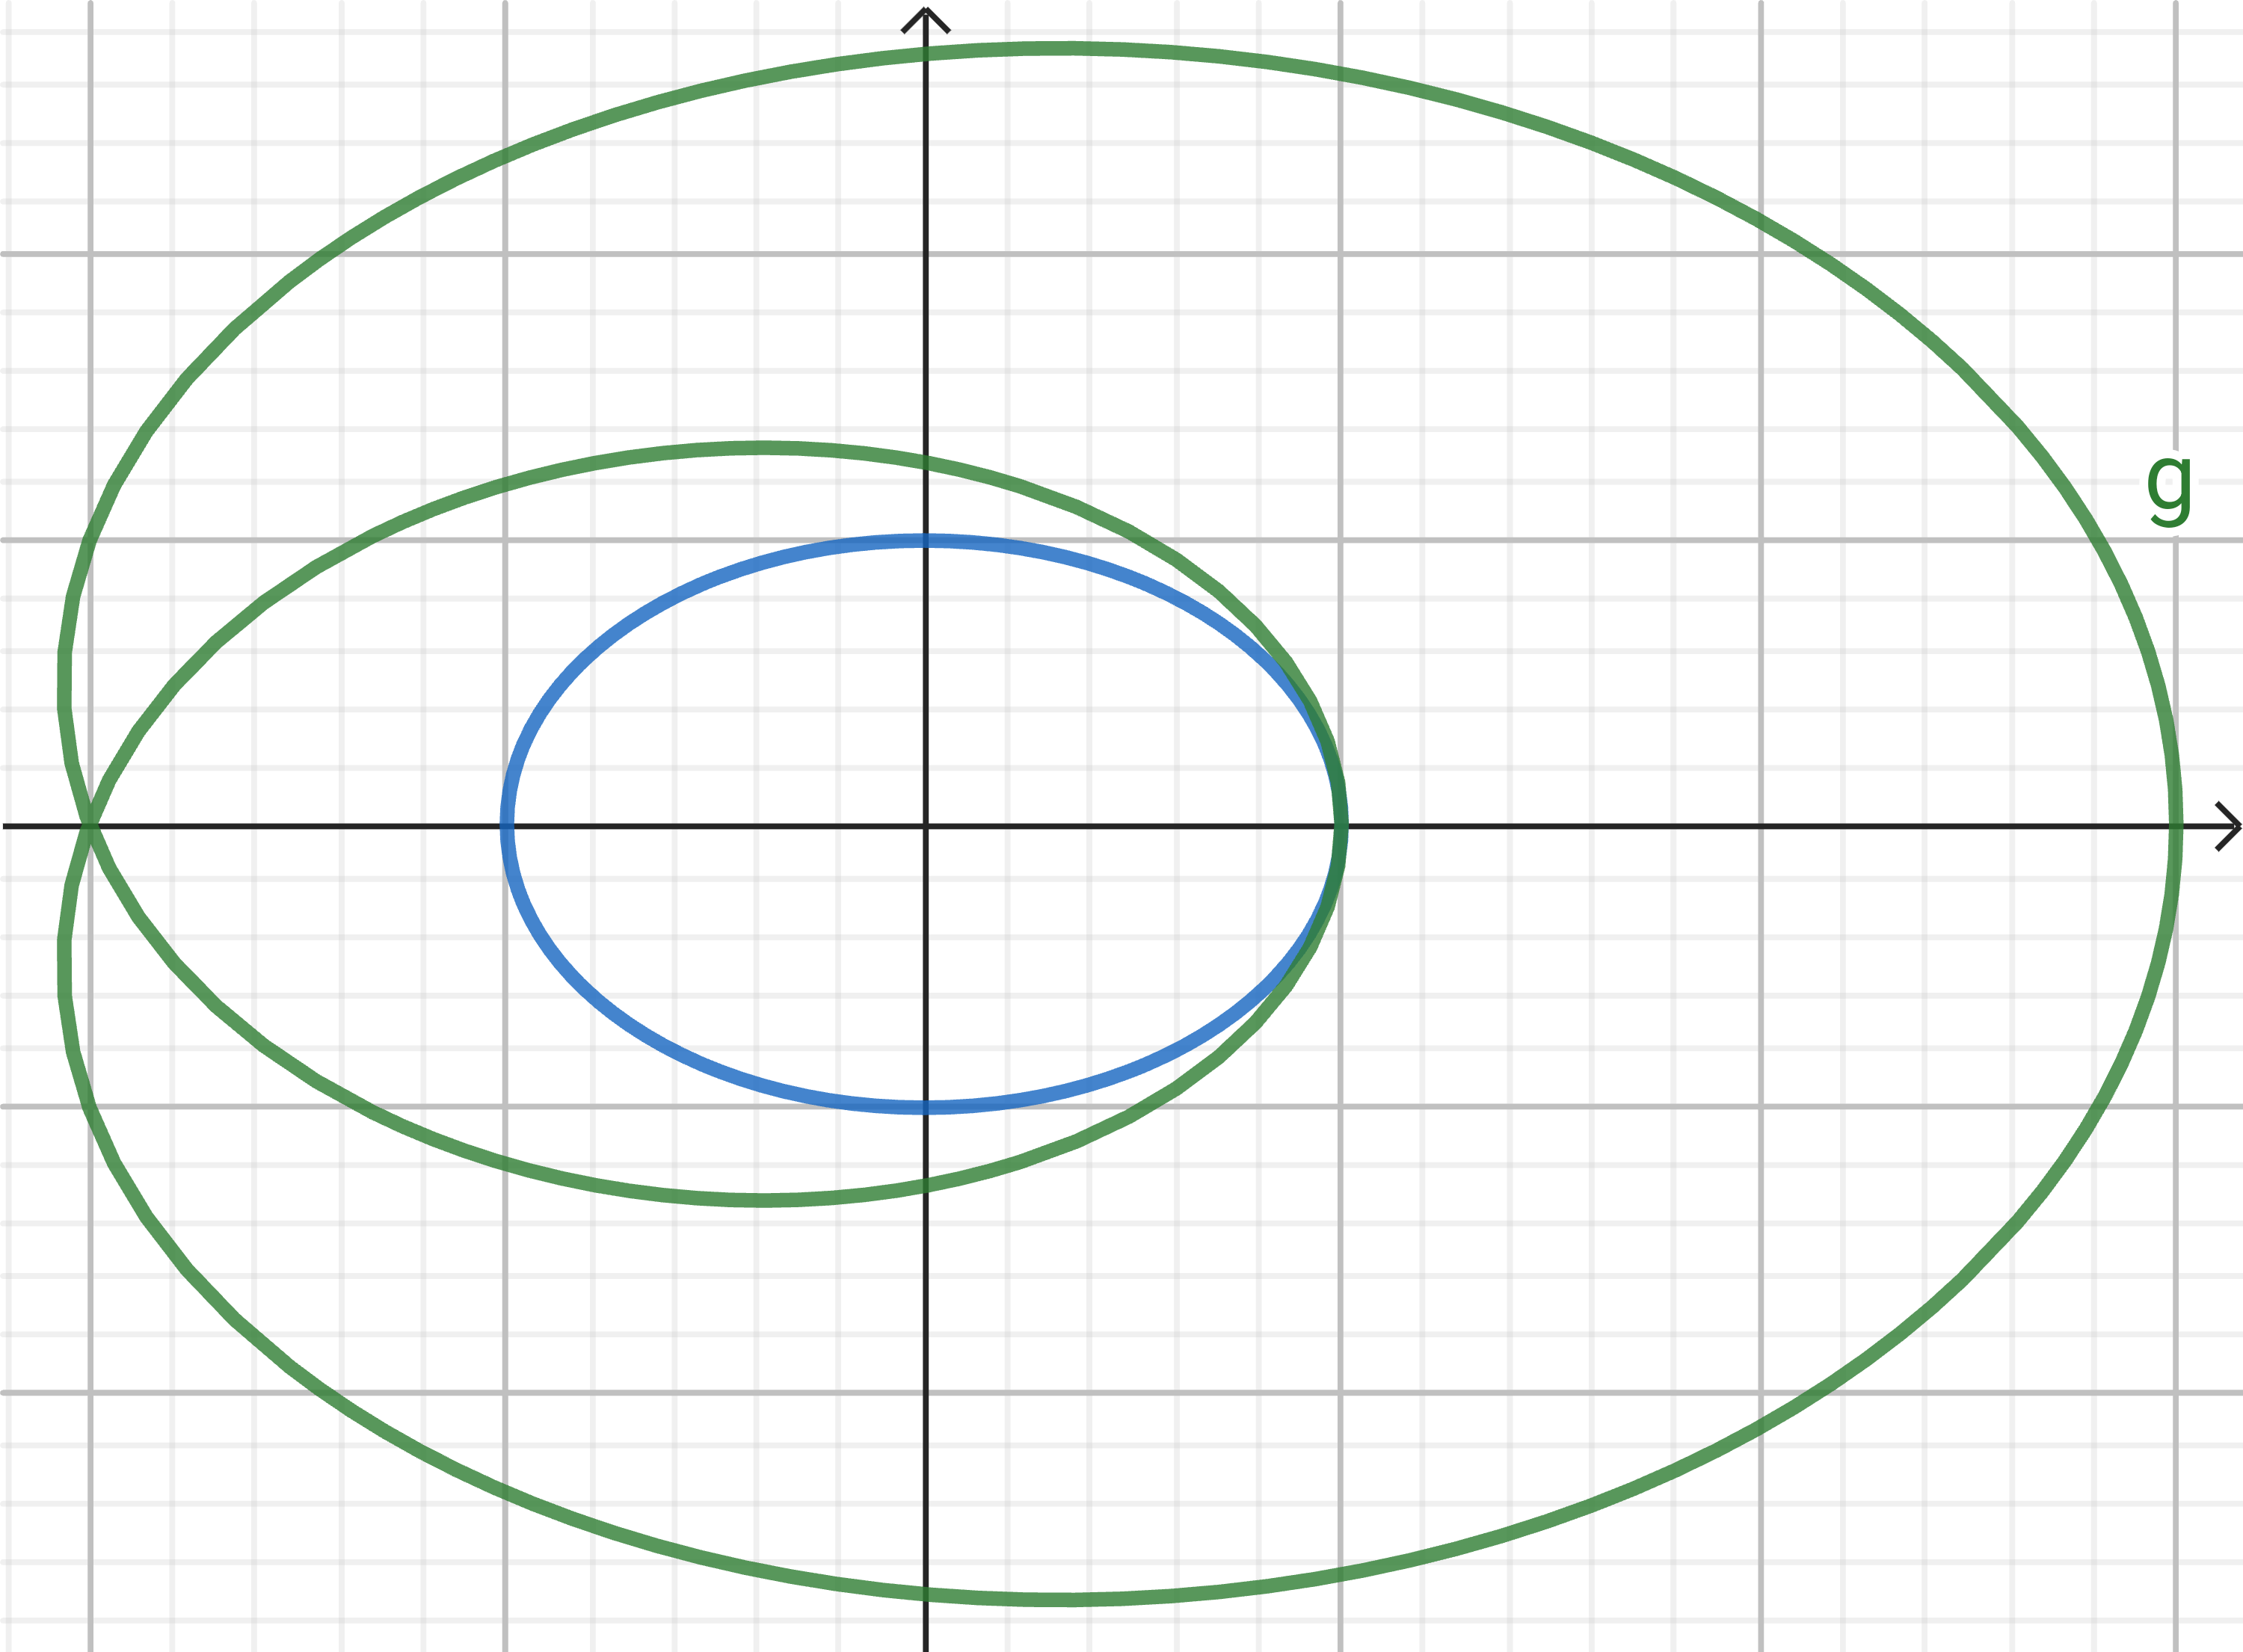
\includegraphics[width = 5cm]{homotopia.png}
\end{figure}

\begin{titlemize}{Lista de consequências}
	\item \hyperref[teo-fundamental-da-algebra]{teo-fundamental-da-algebra};\\ 
	
\end{titlemize}

\subsection{teo-fundamental-da-algebra} %afirmação aqui significa teorema/proposição/colorário/lema
\label{teo-fundamental-da-algebra}
\begin{titlemize}{Lista de dependências}
	\item \hyperref[lema-teo-fundamental-da-algebra]{lema-teo-fundamental-da-algebra};\\ %'dependencia1' é o label onde o conceito Dependência 1 aparece (--à arrumar um padrão para referencias e labels--) 
	\item \hyperref[extensão-da-função-na-esfera]{extensão-da-função-na-esfera};\\
  \item \hyperref[grupo-fundamental-de-S1-prop]{grupo-fundamental-de-S1-prop}
\end{titlemize}
\begin{thm}[Teorema Fundamental da Álgebra]

	Todo polinômio não constante com coeficientes complexos possui raíz em $\mathbb{C}$. \\
 
 Em outras palavras, esse teorema garante que o corpo dos complexos é um fecho algébrico dos corpos de característica 0.
 
\end{thm}

\begin{dem}

Pelo lema referenciado na lista de dependências, basta mostrar que as funções $f_r^n: r\mathbb{S}^1 \rightarrow \mathbb{C}\backslash\{0\}$, definidas por $f_r^n(z) = z^n$, não são homotópicas a uma constante.
De fato, caso $f_r^n$ fosse homotópica a uma constante, então $h: \mathbb{S}^1 \rightarrow r\mathbb{S}^1 \rightarrow \mathbb{C}\backslash\{0\} \rightarrow \mathbb{S}^1$ dada por $h(z) = \frac{f_r^n(rz)}{|f_r^n(rz)|}$ também seria homotópica a uma constante, já que se $H:r\mathbb{S}^1 \times I \rightarrow \mathbb{C}\backslash\{0\}$ é a homotopia entre $f_r^n$ e uma constante $c_0$, então $\frac{1}{r^n}H(rz, t)$ é homotopia entre $h$ e $\frac{c_0}{r^n}$.\\
No entanto, por uma das equivalências de \hyperref[extensão-da-função-na-esfera]{extensão-da-função-na-esfera}, se $h$ é homotópica a uma constante, então $h_*$ é trivial, implicando que $h_*([e^{2\pi i}])$ é elemento neutro em $\mathcal{S}^1$, ou seja $[e^{2\pi in}] = [1]$ e, portanto, com a linguagem do levantamento de homotopia na seção do grupo fundamental de $\mathbb{S}^1$, temos que $deg([e^{2\pi in]}) = deg([1]) = 0$, contrariando o fato de que, na verdade, $deg([e^{2\pi in}]) = n$. Portanto, $f_r^n$ não pode ser homotópico a uma constante e, dessa forma, vale o Teorema Fundamental da Álgebra.

    
\end{dem}

Note que a interpretação geométrica de $h$ é de alongar os pontos em $\mathbb{S}^1$, aumentando o seu raio, e depois rotacioná-los e contraí-los de volta a $\mathbb{S}^1$. A homotopia de $h$ a constante só leva deforma continuamente a circunferência de raio $1$ no ponto $c_0$, trazendo-o mais próximo da origem.

%---------------------------------------------------------------------------------------------------------------------!Draft!-----------------------------------------------------------------------------------------------------------------
\subsection{Identidade e antípoda são homotópicas se há campo não nulo} %afirmação aqui significa teorema/proposição/colorário/lema
\label{identidade-e-antipoda-homotopicas-prop}
\begin{titlemize}{Lista de dependências}
	\item \hyperref[homotopia-def]{Homotopia};\\ %'dependencia1' é o label onde o conceito Dependência 1 aparece (--à arrumar um padrão para referencias e labels--) 
	%\item \hyperref[]{};\\
% quantas dependências forem necessárias.
\end{titlemize}




\begin{lemma}[Funções identidade e antípoda na esfera]% ou af(afirmação)/prop(proposição)/corol(corolário)/lemma(lema)/outros ambientes devem ser definidos no preambulo de Alg.Top-Wiki.tex 
	Se existe uma função contínua $v:S^n\rightarrow \mathbb{R}^{n+1}$ que leva todo $x\in S^n$ em $v(x)$ com $\langle x, v(x) \rangle =0$, isto é, um campo vetorial contínuo não nulo tangente à esfera, então as funções identidade $Id_{S^n}:S^n\rightarrow S^n$ e antípoda $A_{S^n}:S^n\rightarrow S^n$ dada por $A_{S^n}(x)=-x$ para todo $x\in S^n$ são homotópicas.
\end{lemma}
\begin{dem}
    Seja $v:S^n\rightarrow \mathbb{R}^{n+1}$ o campo vetorial contínuo tangente à esfera que é não nulo em todos os pontos e considere a função contínua $H:S^n\times I\rightarrow S^n$ definida por $$H(x,t)=cos(\pi t)x+sen(\pi t)\frac{v(x)}{||v(x)||}.$$
    De fato, $H$ está bem definida pois, utilizando o fato de que $\langle x, v(x) \rangle =0$, temos 

    $$|cos(\pi t)x+sen(\pi t)\frac{v(x)}{||v(x)||}|^2=$$$$=\langle cos(\pi t)x+sen(\pi t)\frac{v(x)}{||v(x)||} , cos(\pi t)x+sen(\pi t)\frac{v(x)}{||v(x)||}\rangle=$$$$=cos^2(\pi t)\langle x,x \rangle +sen^2(\pi t)\langle \frac{v(x)}{||v(x)||},\frac{v(x)}{||v(x)||}\rangle=$$$$=cos^2(\pi t)+sen^2(\pi t)=1.$$
    
    Isto é, $H(x,t)$ pertence à esfera para todo $(x,t)\in X\times I$. Além disso, $H$ é homotopia entre a identidade e a antípoda pois $$H(x,0)=cos(0)x+sen(0)\frac{v(x)}{||v(x)||}=x=Id(x)\text{ para todo } x\in S^n$$ $$\text{e } H(x,1)=cos(\pi)x+sen(\pi)\frac{v(x)}{||v(x)||}=-x=A(x)\text{ para todo }x\in S^n.$$
\end{dem}


\begin{titlemize}{Lista de consequências}
	\item \hyperref[teorema-bola-cabeluda-prop]{Teorema da Bola Cabeluda};\\ %'consequencia1' é o label onde o conceito Consequência 1 aparece
	%\item \hyperref[]{}
\end{titlemize}

%[Bianca]: Um arquivo tex pode ter mais de uma afirmação (ou definição, ou exemplo), mas nesse caso cada afirmação deve ter seu próprio label. Dar preferência para agrupar afirmações que dependam entre sí de maneira próxima (um teorema e seu corolário, por exemplo)

%---------------------------------------------------------------------------------------------------------------------!Draft!-----------------------------------------------------------------------------------------------------------------
\subsection{Teorema da Bola Cabeluda} %afirmação aqui significa teorema/proposição/colorário/lema
\label{teorema-bola-cabeluda-prop}
\begin{titlemize}{Lista de dependências}
	\item \hyperref[homotopia-def]{Homotopia};\\ %'dependencia1' é o label onde o conceito Dependência 1 aparece (--à arrumar um padrão para referencias e labels--) 
	\item \hyperref[identidade-e-antipoda-homotopicas-prop]{Homotopia entre identidade e antípoda};\\
% quantas dependências forem necessárias.
\end{titlemize}


\begin{thm}[Teorema da Bola Cabeluda]% ou af(afirmação)/prop(proposição)/corol(corolário)/lemma(lema)/outros ambientes devem ser definidos no preambulo de Alg.Top-Wiki.tex 
	A esfera $S^n$ possui um campo vetorial contínuo não nulo em todo ponto isto é, existe uma função contínua $v:S^n\rightarrow \mathbb{R}^{n+1}$ que leva todo $x\in S^n$ a $v(x)$ com $\langle x, v(x) \rangle =0$ e $v(x)\ne 0$, se e somente se $n$ é ímpar.\\
\end{thm}
\begin{dem}
    Se $n$ é ímpar, $n=2k-1$ para algum natural $k$ e basta tomar o campo $$v(x_1,~...,~x_{2k})=(-x_2,~x_1,~-x_4,~x_3,~...,~-x_{2k},~x_{2k-1})\text{ para todo }(x_1,~...,~x_{2k})\in S^n.$$
    De fato, a função é contínua, temos $$\langle(-x_2,~x_1,~...,~-x_{2k},~x_{2k-1}), (x_1,~x_2,~...,~x_{2k-1},~x_{2k}) \rangle =$$$$=-x_1x_2+x_1x_2-...-x_{2k-1}x_{2k}+x_{2k-1}x_{2k}=0$$ e vale $v(x)\ne 0$ para todo $x=(x_1,...,x_{2k})\in S^n$ pois $v(x)=(x_1,~x_2,~...,~x_{2k-1},~x_{2k})=0$ somente se $x_i=0$ para todo $i\in {1,~...,~2k}$, isto é, $v(x)=0$ apenas em ponto fora da esfera.\\

    Reciprocamente, se a esfera $S^n$ possui campo vetorial contínuo não nulo em cada ponto conforme condição do enunciado, segundo o lema \ref{identidade-e-antipoda-homotopicas-prop}, existe uma homotopia entre os mapas identidade e antípoda na esfera, o que não pode ocorrer de $n$ for par.

    
\end{dem}

Vale ressaltar que é possível demostrar que de fato não há homotopia entre a identidade e a antípoda em esferas de grau par através da noção de grau de uma função, existente em homologia. Esse tópico não será abordado neste material.

\begin{titlemize}{Lista de consequências}
	\item \hyperref[consequencia1]{Consequência 1};\\ %'consequencia1' é o label onde o conceito Consequência 1 aparece
	%\item \hyperref[]{}
\end{titlemize}

%[Bianca]: Um arquivo tex pode ter mais de uma afirmação (ou definição, ou exemplo), mas nesse caso cada afirmação deve ter seu próprio label. Dar preferência para agrupar afirmações que dependam entre sí de maneira próxima (um teorema e seu corolário, por exemplo)

%%% Local Variables:
%%% mode: LaTeX
%%% TeX-master: "../Alg.Top-Wiki"
%%% End:

\section{Grupo Fundamental}
\label{grupo-fundamental}

\begin{titlemize}{Lista de Dependências}
	\item \hyperref[Homotopia]{homotopia}\\ %homotopia
\end{titlemize}

Considere um espaço topológico com um ponto base fixado. O seu grupo fundamental é o grupo das classes de equivalência (sob homotopia relativa aos extremos) dos laços no espaço saindo do ponto base. Tal grupo armazena certas informações sobre buracos do espaço topologico, e é invariante sobre a equivalência homotópica. Esta é uma ferramenta poderosa para verificar se dois espaços topológicos são homeomorfos. % (homotópicos). %retirei, não entendi o que querem dizer
Veremos como sua construção se dá com mais detalhes.

%---------------------------------------------------------------------------------------------------------------------!Draft!-----------------------------------------------------------------------------------------------------------------
\subsection{Espaço de Laços}
\label{espaco-lacos-def}
\begin{titlemize}{Lista de dependências}
	%\item \hyperref[dependecia1]{Dependência 1};\\ %'dependencia1' é o label onde o conceito Dependência 1 aparece (--à arrumar um padrão para referencias e labels--)
    \item \hyperref[homotopia-relativa-def]{Homotopia Relativa}
	\item \hyperref[homotopia-relaçao-de-equivalencia-prop]{Homotopia é relação de equivalência};\\
% quantas dependências forem necessárias.
\end{titlemize}
\begin{defi}[Espaço de Laços]
	Seja $X$ um espaço topológico e seja $x_0\in X$ um ponto base. O \textbf{espaço de laços} em $X$ que saem de $x_0$ é definido como
\[\Omega(X,x_0) = \left\{\gamma: I \to X ~|~ \gamma\text{ é contínua e }\gamma(0)=\gamma(1)=x_0\right\}.\]
\end{defi}

Investigaremos a fundo o conjunto $\pi_1(X,x_0) = \Omega(X,x_0)/\sim$, onde $\alpha \sim \beta$ se, e somente se, $\alpha$ e $\beta$ são homotópicas relativo a $\partial I = \{0,1\}$.

\begin{titlemize}{Lista de consequências}
	\item \hyperref[homotopia-relaçao-de-equivalencia]{Homotopia como relação de equivalência};\\ %'consequencia1' é o label onde o conceito Consequência 1 aparece
	\item \hyperref[homotopia-teorema-da-bola-cabeluda]{Teorema da bola cabeluda}
\end{titlemize}

%[Bianca]: é mais fácil criar a lista de dependências do que a de consequências.
\subsection{Produto concatenação de caminhos}
\label{Produto-concatenacao-def}
%\begin{titlemize}{Lista de dependências}
	%\item \hyperref[dependecia1]{Dependência 1};\\ % homotopia
%\end{titlemize}
\begin{defi}[Concatenação de caminhos]
	Seja $X$ um espaço topológico, e sejam $\alpha:I\rightarrow X, \beta:I\rightarrow X$ duas funções contínuas tal que $\beta(0)=\alpha(1).$ O produto concatenação de $\alpha$ e $\beta$ é uma função contínua $\alpha*\beta:I\rightarrow X$ dada por 
 \begin{align*}
     (\alpha*\beta)(s)=\begin{cases}
         \alpha(2s)\mbox{ se }0\le s\le\frac{1}{2}\\
         \beta(2s-1)\mbox{ se }\frac{1}{2}\le s \le 1
     \end{cases}
 \end{align*}
\end{defi}

Esse produto será usado para definir o grupo fundamental.

\begin{titlemize}{Lista de consequências}
	%\item \hyperref[consequencia1]{Consequência 1};\\ %'consequencia1' é o label onde o conceito Consequência 1 aparece
	\item \hyperref[produto-bem-definido-prop]{O produto do grupo fundamental}
\end{titlemize}

%[Bianca]: é mais fácil criar a lista de dependências do que a de consequências.

\subsection{O produto do grupo fundamental} %afirmação aqui significa teorema/proposição/colorário/lema
\label{produto-bem-definido-prop}
\begin{titlemize}{Lista de dependências}
	\item \hyperref[Produto-concatenacao-def]{Produto concatenação de caminhos};\\ %'dependencia1' é o label onde o conceito Dependência 1 aparece (--à arrumar um padrão para referencias e labels--) 
% quantas dependências forem necessárias.
\end{titlemize}
Sejam $X$ um espaço topológico e $x_0\in X$. Provemos que o produto concatenação induz um produto $\cdot$ (operação binária) no espaço quociente $\pi_1(X,x_0)$, e que, além disso, $(\pi_1(X,x_0),\cdot)$ é um grupo.

\begin{lemma}% ou af(afirmação)/prop(proposição)/corol(corolário)/lemma(lema)/outros ambientes devem ser definidos no preambulo de Alg.Top-Wiki.tex 
    O produto $\cdot:\pi_1(X,x_0)\times\pi_1(X,x_0)\rightarrow \pi_1(X,x_0)$ dado por $[\alpha]\cdot[\beta]=[\alpha*\beta]$ é bem definido.
\end{lemma}

\begin{dem}
    É claro que o produto concatenação de dois laços em $\Omega(X,x_0)$ ainda é um laço em $\Omega(X,x_0)$. Basta provar que o produto $\cdot$ não depende da escolha de representantes. Sejam $\alpha\sim_H \alpha'$ e $\beta\sim_G\beta'$ laços em $\Omega(X,x_0)$. Então, a função $H*G:I\times I\rightarrow X$ dada por 
    \begin{align*}
        H*G(s,t)=\begin{cases}
            H(2s,t)\qquad&\mbox{ se }0\le s\le \frac{1}{2}\\
            G(2s-1,t)\qquad&\mbox{ se }\frac{1}{2}\le s\le1
        \end{cases}
    \end{align*}
    é uma homotopia satisfazendo $H*G(s,0)=\alpha*\beta(s),$ $H*G(s,1)=\alpha'*\beta'(s)$ e $H*G(0,t)=H*G(1,t)=x_0$ para todos $s,t\in I$. Ou seja, $H*G$ é uma homotopia relativa à $\partial I$ entre $(\alpha*\beta)$ e $(\alpha'*\beta').$ Logo, temos  
    $$[\alpha]\cdot[\beta]=[\alpha*\beta]=[\alpha'*\beta']=[\alpha']\cdot [\beta']$$
    conforme desejado.
\end{dem}

\begin{lemma}
    O produto $\cdot$ é associativo. Ou seja, para todos $\alpha,\beta,\gamma\in\Omega(X,x_0),$ vale
    \[(\alpha*\beta)*\gamma\sim \alpha*(\beta*\gamma).\]
\end{lemma}

\begin{dem}
    Basta exibir uma homotopia entre tais laços. Definimos a função $H:I\times I\rightarrow X$ na seguinte forma:
    \begin{align*}
        H(s,t)=\begin{cases}
            \alpha(\frac{4s}{t+1})\qquad &\mbox{ se }0\le s \le \frac{t+1}{4}\\
            \beta(4s-t-1)\qquad &\mbox{ se }\frac{t+1}{4}\le s\le\frac{t+2}{4}\\
            \gamma(\frac{4s-t-2}{2-t})\qquad &\mbox{ se }\frac{t+2}{4}\le s\le 1.
        \end{cases}
    \end{align*}
    É fácil ver que $H$ é uma homotopia que satisfaz
    \begin{align*}
        H(s,0)=\begin{cases}
            \alpha(\frac{4s}{1})\qquad &\mbox{ se }0\le s \le \frac{1}{4}\\
            \beta(4s-1)\qquad &\mbox{ se }\frac{1}{4}\le s\le\frac{2}{4}\\
            \gamma(\frac{4s-2}{2})\qquad &\mbox{ se }\frac{2}{4}\le s\le 1.
        \end{cases}\quad=((\alpha*\beta)*\gamma)(s),
    \end{align*}
    \begin{align*}
        H(s,1)=\begin{cases}
            \alpha(\frac{4s}{2})\qquad &\mbox{ se }0\le s \le \frac{2}{4}\\
            \beta(4s-2)\qquad &\mbox{ se }\frac{2}{4}\le s\le\frac{3}{4}\\
            \gamma(4s-3)\qquad &\mbox{ se }\frac{3}{4}\le s\le 1.
        \end{cases}\quad=(\alpha*(\beta*\gamma))(s)
    \end{align*}
    e $H(0,t)=H(1,t)=x_0.$ Portanto, $$(\alpha*\beta)*\gamma\sim \alpha*(\beta*\gamma)$$ conforme desejado.
\end{dem}

\begin{lemma}
    Seja $c_{x_0}:I\rightarrow X$ uma função constante cuja valor é igual a $x_0.$ Então, para todo laço $\alpha\in \Omega(X,x_0),$ vale
    $$c_{x_0}*\alpha\sim\alpha\sim\alpha*c_{x_0}.$$
    Ou seja, $[c_{x_0}]$ é o elemento neutro em $(\pi_1(X,x_0),\cdot)$.
\end{lemma}

\begin{dem}
    A homotopia $H$ dada por 
    \begin{align*}
        H(s,t)=\begin{cases}
            x_0\qquad &\mbox{ se }0\le s \le \frac{1-t}{2}\\
            \alpha(\frac{2s-1+t}{1+t}) \qquad &\mbox{ se }\frac{1-t}{2}\le s\le 1
        \end{cases}
    \end{align*}
    é uma homotopia relativa à $\partial I$ entre $c_{x_0}*\alpha$ e $\alpha.$
    
    A homotopia $G$ dada por 
    \begin{align*}
        G(s,t)=\begin{cases}
            \alpha(\frac{2s}{t+1})\qquad &\mbox{ se }0\le s \le \frac{t+1}{2}\\
            x_0\qquad &\mbox{ se }\frac{t+1}{2}\le s \le 1
        \end{cases}
    \end{align*}
    é uma homotopia relativa à $\partial I$ entre $\alpha*c_{x_0}$ e $\alpha.$ Portanto, $$c_{x_0}*\alpha\sim\alpha\sim\alpha*c_{x_0},$$ como queríamos demonstrar.
\end{dem}

\begin{lemma}
    Dado um laço $\alpha \in \Omega(X,x_0)$, vale que $\overline{\alpha}$ dado por $\overline{\alpha}(s)=\alpha(1-s)$ é um laço satisfazendo 
    $$\overline{\alpha}*\alpha\sim c_{x_0}=\alpha*\overline{\alpha}.$$
    Ou seja, $[\overline{\alpha}]$ é o elemento inverso de $[\alpha]$ em $(\pi_1(X,x_0),\cdot)$.
\end{lemma}

\begin{dem}
    A homotopia $H$ dada por 
    \begin{align*}
        H(s,t)=\begin{cases}
            \overline{\alpha}(2s(1-t))\qquad &\mbox{ se }0\le s \le \frac{1}{2}\\
            \overline{\alpha}(2(1-s)(1-t)) \qquad &\mbox{ se }\frac{1}{2}\le s\le 1 
        \end{cases}
    \end{align*}
    é uma homotopia relativa à $\partial I$ entre $\overline{\alpha}*\alpha$ e $c_{x_0},$ porque $H(s,1)=\overline{\alpha}(0)=x_0$ para todo $s\in I$ e 
    \begin{align*}
        H(s,0)=\begin{cases}
            \overline{\alpha}(2s)\qquad &\mbox{ se }0\le s \le \frac{1}{2}\\
            \overline{\alpha}(2(1-s))=\alpha(2s-1) \qquad &\mbox{ se }\frac{1}{2}\le s\le 1
        \end{cases}
    \end{align*}
    (Geometricamente, $H(s,t_0)$ é um laço que anda em $\alpha(s),$ para num certo ponto e faz o caminho de volta).
    De forma análoga, a homotopia $G$ dada por 
   
\begin{align*}
        H(s,t)=\begin{cases}
            \alpha(2s(1-t))\qquad &\mbox{ se }0\le s \le \frac{1}{2} \\
            \alpha(2(1-s)(1-t)) \qquad &\mbox{ se }\frac{1}{2}\le s\le 1 
        \end{cases}
    \end{align*}
    é uma homotopia relativa à $\partial I$ entre $\alpha*\overline{\alpha}$ e $c_{x_0}.$ Portanto, $$\overline{\alpha}*\alpha\sim c_{x_0}=\alpha*\overline{\alpha}$$ conforme desejado.
\end{dem}

Juntando todos os lemas, concluímos: 

\begin{thm}
    Dados $X$ um espaço topológico e $x_0\in X$, vale que $(\pi_1(X,x_0),\cdot)$ é um grupo.
\end{thm}

\begin{titlemize}{Lista de consequências}
	\item \hyperref[grupo-fundamental-def]{Grupo fundamental};\\
    \item \hyperref[conjugacao-por-curva-prop]{Conjugação por uma Curva}
\end{titlemize}

\subsection{Grupo fundamental}
\label{grupo-fundamental-def}
\begin{titlemize}{Lista de dependências}
	\item \hyperref[espaco-lacos-def]{O espaço de laços}
	\item \hyperref[produto-bem-definido-prop]{O produto do grupo fundamental};\\ %'dependencia1' é o label onde o conceito Dependência 1 aparece (--à arrumar um padrão para referencias e labels--) 
% quantas dependências forem necessárias.
\end{titlemize}
\begin{defi}[Grupo fundamental]
	Seja $X$ um espaço topológico e seja $x_0$ um ponto de $X.$ O grupo fundamental de $X$ em $x_0$ é $(\pi_1(X,x_0),\cdot)$, onde $\pi_1(X,x_0) = \Omega(X,x_0)/\sim$, onde $\alpha \sim \beta$ se, e somente se, $\alpha$ e $\beta$ são homotópicas relativo aos extremos, e o produto $\cdot$ é dado por $[\alpha]\cdot\[\beta\] = [\alpha \cdot \beta]$, em que $\alpha \cdot \beta$ é a concatenação de $\alpha$ e $\beta$.
\end{defi}

No geral, o grupo fundamental depende da escolha do ponto base $x_0$.

\begin{titlemize}{Lista de consequências}
	\item \hyperref[hom-grupo-fundamental]{Homomorfismo induzido};\\ %'consequencia1' é o label onde o conceito Consequência 1 aparece
	\item \hyperref[]{}
\end{titlemize}

\subsection{Homomorfismo de grupo fundamental}
\label{hom-grupo-fundamental}
\begin{titlemize}{Lista de dependências}
	\item \hyperref[grupo-fundamental-def]{Dependência 1};\\ %'dependencia1' é o label onde o conceito Dependência 1 aparece (--à arrumar um padrão para referencias e labels--) 
\end{titlemize}
Sejam $X,Y$ espaços topológicos não triviais e $f:X\rightarrow Y$ uma função contínua. Então, $f$ induz uma função entre grupos fundamentais de forma natural:
\begin{align*}
    f_*:\pi_1(X,x_0)&\longrightarrow\pi_1(Y,f(x_0))\\
    [\alpha]\longmapsto [f\circ \alpha].
\end{align*}
É fácil de observar que $f_*$ está bem definida pois se $\alpha\sim \alpha'$ relativa à $\partial I,$ então $f\circ \alpha\sim f\circ \alpha'$ relativa à $\partial I.$ Além disso, se $f\sim g$ relativa à $\partial I$, então $f_*=g_*.$ Agora, provaremos que $f_*$ é um homomorfismo de grupo.
\begin{prop}
    Sejam $X,Y,Z$ espaços topológicos não triviais, e sejam $f:(X,x_0)\rightarrow (Y,y_0)$ e $g:(Y,y_0)\rightarrow (Z,z_0)$ duas funções contínuas que satisfazem $f(x_0)=y_0$ e $g(y_0)=z_0.$ Então, 
    \begin{itemize}
        \item $g_*\circ f_*=(g\circ f)_*;$
        \item $(1_X)_*=1_{\pi_1(X,x_0)};$
        \item $f_*$ é homomorfismo de grupos.
    \end{itemize}
\end{prop}
    
\begin{dem}
    Os dois primeiros itens são triviais. Vamos provar que $f_*$ é homomorfismo. Primeiramente note que 
    \begin{align*}
        f\circ (\alpha*\beta)(s)=\begin{cases}
            f(\alpha(2s))&\;\;\;\mbox{ se }0\le s\le \frac{1}{2}\\
            f(\beta(2s-1))&\;\;\;\mbox{ se }\frac{1}{2}\le s\le 1
        \end{cases}\;\;\;\;= ((f\circ\alpha)*(f\circ \beta))(s)
    \end{align*}
    Logo, temos
    \begin{align*}
        f_*([\alpha]\cdot [\beta])=f_*[\alpha*\beta]=[f\circ (\alpha*\beta)]=[(f\circ\alpha)*(f\circ\beta)]=(f_*[\alpha])\cdot (f_*[\beta])
    \end{align*}
    conforme desejado.
\end{dem}

Podemos concluir que na linguagem da teoria de categorias, $\pi_1$ é um funtor de $\textbf{Top}^*$ em \textbf{Gr}. 

Como consequência, temos que $\pi_1(X,x_0)$ é invariante topológico.

\begin{corol}
    Se $f:X\rightarrow Y$ é homeomorfismo, então $f_*:\pi_1 (X,x_0)\rightarrow \pi_1(Y,f(x_0))$ é um isomorfismo de grupos.
\end{corol}

\begin{dem}
    Seja $g:Y\rightarrow X$ a inversa de $f.$ Pela proposição anterior, temos que 
    $$f_*\circ g_*=(f\circ g)_*=(1_Y)_*=1_{\pi_1(Y,f(x_0))}$$
    e 
    $$g_*\circ f_*=(g\circ f)_*=(1_X)_*=1_{\pi_1 (X,x_0)}.$$
    Portanto, $f_*$ é um isomorfismo de grupo.
\end{dem}

\begin{titlemize}{Lista de consequências}
	\item \hyperref[consequencia1]{Consequência 1};\\ %'consequencia1' é o label onde o conceito Consequência 1 aparece
	\item \hyperref[]{}
\end{titlemize}

%---------------------------------------------------------------------------------------------------------------------!Draft!-----------------------------------------------------------------------------------------------------------------
\subsection{Conjugação por uma Curva} %[conjugacao-por-curva-prop]{Conjugação por uma Curva}
\label{conjugacao-por-curva-prop}
\begin{titlemize}{Lista de dependências}
    \item \hyperref[espaco-lacos-def]{Espaço de Laços};\\
    \item \hyperref[produto-bem-definido-prop]{O produto do grupo fundamental};\\
	\item \hyperref[grupo-fundamental-def]{O Grupo Fundamental};
% quantas dependências forem necessárias.
\end{titlemize}
%Comentário sobre os objetos envolvidos na afirmação.
\begin{defi}[Conjugação de laços por uma curva] 
	Sejam $x_0$ e $x_1$ pontos em um espaço topológico $X$ e seja $\gamma: I \to X$ uma curva contínua ligando $x_0$ a $x_1$; isto é, $\gamma(0)=x_0$ e $\gamma(1) = x_1$. Seja também $\eta \in \Omega(X,x_0)$ um laço saindo de $x_0$. Definimos a conjugação de $\eta$ por $\gamma$ como $\overline{\gamma} * \eta * \gamma \in \Omega(X,x_1)$, laço saindo de $x_1$. Isto define uma função $A_{\gamma}: \Omega(X,x_0) \to \Omega(X,x_1)$.
\end{defi}

\begin{prop}[Isomorfismo de grupos induzido por $A_{\gamma}$]
    Sejam $x_0$ e $x_1$ pontos em um espaço topológico $X$ e seja $\gamma: I \to X$ uma curva ligando $x_0$ a $x_1$.
    
    Então $A_{\gamma}$ induz um isomorfismo de grupos \begin{align*}
        \hat{A}_{\gamma}: \pi_1(X,x_0)&\to \pi_1(X,x_1)\\
        \hat{A}_{\gamma}([\eta]) &= [A_{\gamma}(\eta)] = [\overline{\gamma} * \eta * \gamma].
    \end{align*}

    \begin{dem}
        Provemos primeiramente que $\hat{A}_{\gamma}$ está bem definida. Considere $c_{\gamma}: \gamma \Rightarrow \gamma$ e $c_{\overline{\gamma}}: \overline{\gamma} \Rightarrow \overline{\gamma}$ as homotopias constantes. Assim, se $\eta, \nu \in \Omega(X,x_0)$ e $H: \eta \Rightarrow \nu$ é uma homotopia relativa a $\partial I$ então é claro que $c_{\overline{\gamma}}*H*c_{\gamma}: A_{\gamma}(\eta) \Rightarrow A_{\gamma}(\nu)$ também é homotopia relativa a $\partial I$.

        $\hat{A}_{\gamma}$ é um homomorfismo de grupos, já que dadas $\eta, \nu \in \Omega(X,x_0)$,
        \begin{align*}
            \hat{A}_{\gamma}([\eta]\cdot[\nu]^{-1})
            &= \hat{A}_{\gamma}([\eta * \overline{\nu}])\\
            &= [\overline{\gamma} * (\eta * \overline{\nu}) * \gamma]\\
            &= [(\overline{\gamma} * \eta * \gamma)*(\overline{\gamma} * \overline{\nu} * \gamma)]\\
            &= [\overline{\gamma} * \eta * \gamma]\cdot[\overline{\overline{\gamma} * \nu * \gamma}]\\
            &= \hat{A}_{\gamma}([\eta]) \cdot \hat{A}_{\gamma}([\nu])^{-1}.
        \end{align*}
        
        Por fim, note que $\hat{A}_{\gamma}$ e $\hat{A}_{\overline{\gamma}}$ são inversas, pois \[A_{\gamma} \circ A_{\overline{\gamma}}(\eta) = (\overline{\gamma} * \gamma) * \eta * (\overline{\gamma} * \gamma) \sim \eta\text{ relativa a }\partial I\]
        para toda curva $\gamma: I \to X$. Desse modo $\hat{A}_{\gamma}$ é um isomorfismo de grupos.
    \end{dem}
\end{prop}

Um fato importante decorrente de tal proposição é o seguinte.

\begin{corol}
    Se $X$ é um espaço topológico então $\pi_1(X,x_0)$ é isomorfo a $\pi_1(X,x_1)$, para quaisquer $x_0, x_1 \in X$ na mesma componente conexa por caminhos de $X$. Em especial, o grupo fundamental independe do ponto base caso $X$ seja conexo por caminhos.
\end{corol}

\begin{nota}
    Sejam $X$ e $Y$ espaços topológicos, $x_0, x_1\in X$ e $\gamma:I\to X$ uma curva ligando $x_0$ a $x_1$. Seja também $f: X\to Y$ uma função contínua e denotemos $y_0 = f(x_0)$ e $y_1 = f(x_1)$. Então $f(\gamma):I \to Y$ liga $y_0$ a $y_1$, e vale que
    \[f_{*,x_1} \circ \hat{A}_{\gamma} = \hat{A}_{f(\gamma)} \circ f_{*,x_0}.\]
    \begin{dem}
        Para cada $\eta \in \Omega(X,x_0)$,
        \begin{align*}
            \hat{A}_{f(\gamma)} \circ f_{*,x_0}([\eta])
            &= \hat{A}_{f(\gamma)} ([f(\eta]))\\
            &= [\overline{f(\gamma)} * f(\eta) * f(\gamma)]\\
            &= [f(\overline{\gamma}) * f(\eta) * f(\gamma)]\\
            &= [f(\overline{\gamma} * \eta * \gamma)]\\
            &= [f(A_{\gamma}(\eta)]
            = f_{*,x_1}\circ \hat{A}_{\gamma}([\eta]).
        \end{align*}
    \end{dem}
\end{nota}

\begin{titlemize}{Lista de consequências}
	\item \hyperref[equiv-homotopia-induz-iso]{Equivalência de homotopia e o grupo fundamental};\\ %'consequencia1' é o label onde o conceito Consequência 1 aparece
	%\item \hyperref[]{}
\end{titlemize}

%[Bianca]: Um arquivo tex pode ter mais de uma afirmação (ou definição, ou exemplo), mas nesse caso cada afirmação deve ter seu próprio label. Dar preferência para agrupar afirmações que dependam entre sí de maneira próxima (um teorema e seu corolário, por exemplo)

\subsection{Equivalência de homotopia e o grupo fundamental}
\label{equiv-homotopia-induz-iso}
\begin{titlemize}{Lista de dependências}
    \item \hyperref[equiv-homotopia]{Equivalência de Homotopia};
	\item \hyperref[hom-grupo-fundamental]{Homomorfismo de grupos fundamentais};
    \item \hyperref[conjugacao-por-curva-prop]{Conjugação por uma Curva}
\end{titlemize}

\begin{lemma}
    Sejam $X$ um espaço topológico, $x_0\in X$ e $\phi: X \to X$ uma função contínua tal que $\phi\sim \text{id}_X$. Então $\phi_*: \pi_1(X,x_0)\to \pi_1(X,\phi(x_0))$ é isomorfismo de grupos.

    \begin{dem}
        Denotemos $x_1=\phi(x_0)$. Tomemos $H(x,t): X\times I \to X$ uma homotopia de $\text{id}_X$ à $\phi$. Então a curva $\gamma: I \to X$ dada por $\gamma(t) = H(x_0,t)$ liga $x_0$ a $x_1$.
        
        Afirmamos que $\phi_* = \hat{A}_{\gamma}$; ou seja, para toda $\eta \in \Omega(X,x_0)$ vale que $\phi(\eta) \sim \overline{\gamma} * \eta * \gamma$ relativa a $\partial I$. De fato, $H(\eta(.),.): I\times I \to X$ é contínua, $H(\eta(s),0)=\eta(s)$ e $H(\eta(s),1)=\phi(\eta)(s)$ para todo $s\in I$, sendo assim uma homotopia entre $\eta$ e $\phi(\eta)$. Definindo então\begin{align*}
            H': I\times I&\to X\\
                (s,t)&\mapsto \begin{cases}
                \overline{\gamma}(s),&\text{ se }s\in[0,\frac{t}{3}]\\
                H\left(\eta\left(\frac{3s-t}{3-2t}\right),t\right),&\text{ se }s\in[\frac{t}{3},1-\frac{t}{3}]\\
                \gamma(s),&\text{ se }s\in[1-\frac{t}{3},1]
            \end{cases}
        \end{align*}
        concluímos que $\phi(\eta) \underset{H'}{\sim} \overline{\gamma} * \eta * \gamma$ relativa a $\partial I$.
    \end{dem}
\end{lemma}


\begin{thm}
    Sejam $X$ e $Y$ espaços topológicos, $x_0\in X$ e $f:X\to Y$ uma equivalência de homotopia. Então, $f_*: \pi_1(X,x_0) \to \pi_1(X,f(x_0))$ é isomorfismo de grupos.
\end{thm}

Tal resultado não é tão imediato quanto se parece. Tomando $g: Y\to X$ inversa a menos de homotopia de $f$, $g \circ f \sim \text{id}_X$, porém disso não segue que $f_* \circ g_* = \text{id}_{\pi_1(X,x_0)}$, pois $g_* \circ f_*: \pi_1(X,x_0) \to \pi_1(X,g\circ f(x_0))$. E mesmo que $g\circ f(x_0) = x_0$, a homotopia $H: g\circ f\Rightarrow \text{id}_X$ não precisa ser relativa à $\{x_0\}$.

\begin{dem}
    Sejam $y_0 = f(x_0)$, $x_1 = g(y_0) = g\circ f(x_0)$ e $y_1 = f(x_1) = f\circ g\circ f(x_0)$. Sabemos que as composições
    \[\pi_1(X,x_0) \xrightarrow{f_{*,x_0}} \pi_1(Y,y_0) \xrightarrow{g_{*,y_0}}\pi_1(X,x_1)\]
    e
    \[\pi_1(Y,y_0) \xrightarrow{g_{*,y_0}} \pi_1(X,x_1) \xrightarrow{f_{*,x_1}}\pi_1(Y,y_1)\]
    são homotópicas a $\text{id}_X$ e $\text{id}_Y$, respectivamente. Com tal notação, explicitamos que $f_{*,x_0}$ e $f_{*,x_1}$ estão definidas sobre domínios diferentes. Pelo Lema anterior, $g_{*,y_0}\circ f_{*,x_0}$ e $f_{*,x_1}\circ g_{*,y_0}$ são isomorfismos de grupos. Em especial, $f_{*,x_0}$ é injetora e $f_{*,x_1}$ é sobrejetora.

    Porém a Nota na Seção Conjugação por uma Curva nos garante que $f_{*,x_0} = \hat{A}_{f(\gamma)}^{-1} \circ f_{*,x_1} \circ \hat{A}_{\gamma}$ é composição de funções sobrejetoras, portanto é sobrejetora também (o mesmo argumento garante que $f_{*,x_1}$ é injetora). Como já sabíamos que $f_{*,x_0}$ é homomorfismo de grupos, concluímos que $f_{*,x_0}:\pi_1(X,x_0)\to \pi_1(Y,y_0)$ é isomorfismo de grupos.
\end{dem}


%\begin{titlemize}{Lista de consequências}
	%\item \hyperref[consequencia1]{Consequência 1};\\ %'consequencia1' é o label onde o conceito Consequência 1 aparece
	%\item \hyperref[]{}
%\end{titlemize}

\subsection{grupo-fundamental-convexo}
\label{grupo-fundamental-convexo}
\begin{itemize}{Lista de dependências}
    \item \hyperref[grupo-fundamental]{Dependência 1}
    \item \hyperref[homotopia]{Dependência 2}
    
\end{itemize}
O grupo fundamental de um convexo é sempre trivial. Seja $\alpha$ um laço em um espaço topológico $X$ começando em um ponto $x_0$.
Tomando a homotopia $F:I \times I \longrightarrow X$, onde $F(s,t) = (1 - t)\alpha(s) + tx_0$, teremos que $\pi_1(X, x_0) = \{1\}$.

\begin{itemize}{lista de consequências}
    \item \hyperref[teo-ponto-fixo-Brower]{Consequência 1}
    \item \hyperref[]{}
\end{itemize}

%%% Local Variables:
%%% mode: LaTeX
%%% TeX-master: "../Alg.Top-Wiki"
%%% End:

\section{Espaço de recobrimento}
\label{espaco-de-recobrimento}

\begin{titlemize}{Lista de Dependências}
	\item \hyperref[homotopia]{Homotopia};\\ %homotopia
	\item \hyperref[grupo-fundamental]{Grupo fundamental};\\
    \item \hyperref[topologia-quociente]{Espaço quciente};
\end{titlemize}

Na topologia algébrica, espaços de recobrimento estão intimamente relacionados ao grupo fundamental: Todos os recobrimentos têm a propriedade de levantamento de curva e homotopia, portanto ao invés de acha uma homotopia em espaço original podemos verificar se existir uma homotopia num recobrimento que têm melhores propriedades topológicas. Por isso, os espaços de recobrimento são uma ferramenta importante no cálculo de grupos fundamentais.
\subsection{Espaço de recobrimento}
\label{espaco-de-recobrimento-def}
\begin{titlemize}{Lista de dependências}
	\item \hyperref[topologia-quociente]{Espaço quciente};\\ %'dependencia1' é o label onde o conceito Dependência 1 aparece (--à arrumar um padrão para referencias e labels--) 
% quantas dependências forem necessárias.
\end{titlemize}
\begin{defi}[Espaço de recobrimento]
Uma função contínua $p:E\rightarrow X$ é um \textbf{recobrimento} se para todo $x\in X,$ existe uma vizinhança aberta $U\subseteq X$ de $x$ e um conjunto de índices $\Lambda\ne \varnothing$ tal que 
$$p^{-1}(U)=\amalg_{\lambda\in \Lambda} V_\lambda,$$
onde $V_\lambda\subseteq E$ é um subconjunto aberto e $p|_{V_\lambda}:V_\lambda\rightarrow U$ é homeomorfismo.
\end{defi}

\begin{nota}
Introduzimos algumas terminologias: 
    \begin{itemize}
        \item $E$ é um espaço (total) de recobrimento.
        \item $U$ é um aberto uniformemente recoberto de $X.$
        \item $V_\lambda$ é uma placa de $U$ do recobrimento.
        \item A cardinalidade de $\Lambda$ é o número de folhas do recobrimento (veremos que $\# \Lambda$ não depende de $x$). 
    \end{itemize}
\end{nota}

\begin{ex}
A função $p:\mathbb{R}\rightarrow \mathbb{S}^1$ dada por $p(x)=e^{2\pi ix}$ é um recobrimento: dado $y_0=e^{2\pi i x_0}\in\mathbb{S}^1,$ e $U=\mathbb{S}^1\setminus \{-y_0\}$ nós temos 
$$p^{-1}(U)=\amalg_{k\in \mathbb{Z}} (x_0+\frac{2k-1}{2},x_0+\frac{2k+1}{2}),$$
denotamos intervalo aberto $(x_0+\frac{2k-1}{2},x_0+\frac{2k+1}{2})$ por $V_k.$ Logo, a função $p|_{V_k}:V_k\rightarrow \mathbb{S}^1\setminus\{-y\}$ é um homeomorfismo.
\end{ex}

\begin{ex}
    A função $p:\mathbb{S}^n\rightarrow \mathbb{RP}^n=\mathbb{S}^n/\mathbb{Z}_2$ dada por $p(x)=[x]$ é um recobrimento.
\end{ex}

\begin{ex}
    Dado um conjunto $\Lambda\ne \varnothing$ qualquer munido com a topologia discreta, a função projeção $pr_2:E=\Lambda\times X\rightarrow X$ é um recobrimento. Esse recobrimento é dito \textbf{recobrimento trivial}
\end{ex}

\begin{prop}
    Suponha que $X$ é um espaço topológico conexo e $p:E\rightarrow X$ um recobrimento, então toda fibra tem a mesma cardinalidade, i.e. $\# p^{-1}(x_0)=\# p^{-1}(x_1)$ para todo $x_0,\;x_1\in X.$ Isso mostra que $\Lambda$ não depende de $x$.
\end{prop}

\begin{dem}
    Seja $x_0\in X$ e seja $A=\{x_1\in X: \#p^{-1}(x_1)=\# p^{-1}(x_0)\}.$ O conjunto $A$ não é vazio, pois $x_0\in A.$ Agora vamos provar que $A$ é aberto. Suponha que $x\in A$ e seja $U$ uma vizinhança aberta de $x$ tal que $p^{-1}(U)=\amalg_{\lambda\in \Lambda} V_\lambda$ com $p|_{V_\lambda}:V_\lambda\rightarrow U$ hemeomorfismo. Então, $U\subseteq A,$ pois se $x'\in U,$ então 
    $$\# p^{-1}(x')=\# \Lambda=\# p^{-1}(x)=\# p^{-1}(x_0).$$
    O conjunto $A$ é fechado, pois $X\setminus A$ é aberto pelo mesmo argumento acima. Como $X$ é conexo, $X=A$ como queríamos. 
\end{dem}

\begin{nota}
    Localmente todo recobrimento $p:E\rightarrow U$ é isomorfo ao recobrimento trivial, i.e. para todo $x\in X,$ existem uma vizinhança aberta $U$ de $x$, um espaço topológico discreto $\Lambda,$ e um homeomorfismo $h: E|_U\rightarrow U\times \Lambda$ tal que $pr_1\circ h= p.$
\end{nota}

\begin{titlemize}{Lista de consequências}
	\item \hyperref[levantamento-de-caminhos-prop]{Levantamento de caminhos};\\ %'consequencia1' é o label onde o conceito Consequência 1 aparece
	\item \hyperref[levantamento-de-homotopia-prop]{Levantamento de homotopia};\\
 	\item \hyperref[base-para-topologias-em-recobrimento-prop]{Base para as topologias em um recobrimento};\\
  	\item \hyperref[homomorfismo-induzido-por-recobrimento-prop]{Homomorfismo induzido por recobrimento é injetor};\\
   	\item \hyperref[recobrimento-1-conexo-prop]{Recobrimento 1-conexo quando X slsc}
\end{titlemize}

\subsection{Levantamento de caminhos} %afirmação aqui significa teorema/proposição/colorário/lema
\label{levantamento-de-caminhos-prop}
\begin{titlemize}{Lista de dependências}
	\item \hyperref[espaco-de-recobrimento-def]{Espaço de recobrimento};\\ %'dependencia1' é o label onde o conceito Dependência 1 aparece (--à arrumar um padrão para referencias e labels--) 
	\item \hyperref[]{};\\
% quantas dependências forem necessárias.
\end{titlemize}
\begin{thm}[Levantamento de caminhos]% ou af(afirmação)/prop(proposição)/corol(corolário)/lemma(lema)/outros ambientes devem ser definidos no preambulo de Alg.Top-Wiki.tex
Suponha que $p:E\rightarrow X$ é um recobrimento e $\alpha:I\rightarrow X$ é um caminho com $\alpha(0)=x_0.$ Dado $e_0\in E$ com $p(e_0)=x_0,$ existe um único levantamento $\Tilde{\alpha}_{e_0}:I\rightarrow E$ tal que $p\circ\Tilde{\alpha}_{e_0}=\alpha$ e $\Tilde{\alpha}(0)=e_0.$
\end{thm}

\begin{dem}
    Note que $\alpha(I)$ é compacto, pois $I$ é compacto e $\alpha$ é contínua. Recubra $\alpha(I)\subseteq X$ por abertos uniformemente recobertos e tome uma sub-cobertura finita
    \[\alpha(I)=\bigcup_{i=0}^k U_i. \]
    Pelo lema de Lebesgue, podemos escolher $0=t_0< t_1<...<t_m=1$ tais que $\alpha([t_i,t_{i+1}])\subseteq U_j$ para algum $j.$ 
    
    Indutivamente defina: 
    \begin{enumerate}
        \item Passo inicial: Tome um aberto uniformemente recoberto $U_i$ que contém $\alpha([0,t_1]),$ e tome uma placa $V_i$ de $U_i$ que contém $e_0.$ Defina $\Tilde{\alpha}^1:[0,t_1]\rightarrow E$ com $\Tilde{\alpha}^1=p|_{V_i}^{-1}\circ \alpha|_{[0,t_1]}.$
        \item Passo indução: Assuma que definimos $\Tilde{\alpha}^{j-1}:[0,t_{j-1}]\rightarrow E.$ Então $\Tilde{\alpha}^j:[0,t_j]\rightarrow E$ é definida com 
        \begin{align*}
            \begin{cases}
                \Tilde{\alpha}^j|_{[0,t_{j-1}]}=\Tilde{\alpha}^{j-1}\\
                \Tilde{\alpha}^j|_{[t_{j-1},t_j]}=p|_{V_{j-1}}^{-1}\circ \alpha|_{[t_{j-1},t_j]},
            \end{cases}
        \end{align*}
        onde $V_{j-1}$ é uma placa de um aberto uniformemente recoberto que cobre $\alpha([t_{j-1},t_j]).$
        \item Passo final: definimos $\Tilde{\alpha}_{e_0}:=\Tilde{\alpha}^m.$
    \end{enumerate}

    Essa curva é contínua, pois é localmente contínua e continuidade é uma propriedade local. E é única, pois se $\Tilde{\alpha}_{e_0}':I\rightarrow E$ também satisfaz $p\circ\Tilde{\alpha}_{e_0}'=\alpha$ e $\Tilde{\alpha}'(0)=e_0,$ então, pela definição de recobrimento, para cada $t\in I$ existe um aberto $J$ tal que $\Tilde{\alpha}_{e_0}(t)=\Tilde{\alpha}_{e_0}'(t)$ para todo $t\in J$. Como $I$ é conexo, as curvas $\Tilde{\alpha}_{e_0}$ e $\Tilde{\alpha}_{e_0}'$ coincidem em todos pontos.
\end{dem}

\begin{titlemize}{Lista de consequências}
	\item \hyperref[levantamento-de-homotopia-prop]{Levantamento de Homotopia};\\ %'consequencia1' é o label onde o conceito Consequência 1 aparece
	\item \hyperref[]{}
\end{titlemize}

\subsection{Levantamento de Homotopia} %afirmação aqui significa teorema/proposição/colorário/lema
\label{levantamento-de-homotopia-prop}
\begin{titlemize}{Lista de dependências}
	\item \hyperref[espaco-de-recobrimento-def]{Espaço de recobrimento};\\ %'dependencia1' é o label onde o conceito Dependência 1 aparece (--à arrumar um padrão para referencias e labels--) 
	\item \hyperref[homotopia]{Homotopia};\\
    \item \hyperref[grupo-fundamental]{Grupo fundamental}\\
    \item \hyperref[levantamento-de-caminhos-prop]{Levantamento de caminhos}
% quantas dependências forem necessárias.
\end{titlemize}

\begin{thm}[Levantamento de Homotopia]% ou af(afirmação)/prop(proposição)/corol(corolário)/lemma(lema)/outros ambientes devem ser definidos no preambulo de Alg.Top-Wiki.tex 
	Seja $p:E\rightarrow X$ um recobrimento, e seja $H:I\times I\rightarrow X$ uma homotopia tal que $H(s,0)=\gamma:I\rightarrow X.$ Suponha que $\Tilde{\gamma}:I\rightarrow E$ é um levantamento de $\gamma,$ então existe uma única homotopia $\Tilde{H}:I\times I\rightarrow E$ tal que $\Tilde{H}(s,0)=\Tilde{\gamma}$ e $p\circ \Tilde{H}=H.$
\end{thm}

\begin{dem}
    Note que para cada $s\in I$ fixo, $\alpha^s(t):=H(s,t)$ é uma curva, logo existe um único levantamento $\tilde{\alpha}_{\tilde{\gamma}(s)}(t)$ que começa em ponto $\tilde{\gamma}(s).$ Definimos $\Tilde{H}(s,t):=\Tilde{\alpha}_{\tilde{\gamma}}(t),$ é claro que 
\[p\circ\tilde{H}(s,t)=\alpha^s (t)=H(s,t)\]
e 
\[\tilde{H}(s,0)=\Tilde{\alpha}_{\tilde{\gamma}}(0)=\tilde{\gamma}(s).\]
A unicidade segue que da unicidade do levantamento de caminhos. Pela definição de recobrimento, para cada $(s_0,t_0)\in I\times I$ existe um aberto uniformemente recoberto $U$ contendo $H(s_0,t_0)$ tal que $\tilde{H}|_M=p|_V^{-1}\circ H|_M,$ onde $V$ é uma placa de $U$ e $M=H^{-1}(U).$ Como $H$ e $p|_V^{-1}$ são contínuas e $M$ é aberto, $\tilde{H}$ é localmente contínua, e portanto contínua.
\end{dem}

\begin{corol}
    Sejam $\alpha,\;\beta:I\rightarrow X$ duas curvas. Então, $\alpha$ e $\beta$ são homotópicas relativa a $\partial I$ se, e somente se, os levantamentos $\Tilde{\alpha}_{e_0}$ e $\Tilde{\beta}_{e_0}$ são homotópicos relativo a $\partial I.$ 
\end{corol}

\begin{dem}
    Assuma que $\Tilde{H}$ é homotopia relativa a $\partial I$ dos levantamentos, então $p\circ\Tilde{H}$ é uma homotopia relativa a $\partial I.$ Vamos mostrar a recíproca. Seja $H:\alpha\Rightarrow \beta$ uma homotopia relativa a $\partial I$ e seja $\Tilde{H}:I\times I\rightarrow E$ levantamento de $H$. Temos que mostra:
    \begin{enumerate}
        \item $\tilde{H}(s,1)=\tilde{\beta}_{e_0}(s)$, i.e., $\tilde{H}:\tilde{\alpha}_{e_0}\Rightarrow\tilde{\beta}_{e_0}$ é uma homotopia.
        \item $\tilde{H}(0,t)=e_0$ para todo $t\in I$ e $\tilde{H}(1,t)=\tilde{\alpha}_{e_0}(1)=\tilde{\beta}_{e_0}(1)$ para todo $t\in I,$ i.e., $\tilde{H}:\tilde{\alpha}_{e_0}\Rightarrow\tilde{\beta}_{e_0}$ é relativa a $\partial I.$
    \end{enumerate}
    Como $\tilde{H}(s,1)$ é um levantamento de $\beta$ que começa em $e_0,$ por unicidade de levantamento, $\tilde{H}(s,1)=\tilde{\beta}_{e_0}.$ Por mesmo argumento, como $\tilde{H}(0,t)$ é um levantamento da curva constante igual à $\alpha(0)$ começando em $e_0,$ $\tilde{H}(0,t)=e_0$ para todo $t\in I.$ De forma análoga, $\tilde{H}(1,t)=\tilde{\alpha}_{e_0}(1)=\tilde{\beta}_{e_0}(1)$ para todo $t\in I.$ A demonstração está completa agora. 
\end{dem}

\begin{corol}
    Seja $p:E\rightarrow X$ um recobrimento, e sejam $\alpha,\;\beta:I\rightarrow X$ duas curvas. Se $E$ é 1-conexo, então duas curvas $\alpha,\;\beta$ são homotópica relativa a $\partial I$ se, e somente se, $\tilde{\alpha}_{e_0}(1)=\tilde{\beta}_{e_0}(1).$
\end{corol}

\begin{dem}
    A demonstração segue da definição de 1-conexo.
\end{dem}

Mostraremos um corolário bem útil em calcular grupo fundamental de um espaço topológico.

\begin{corol}\label{cor:bijedeggene}
    Seja $p:E\rightarrow X$ um recobrimento. Se $E$ é 1-conexo, então para cada pontos fixos $x\in X$ e $e\in p^{-1}(x)$, a função dada por 
    \begin{align*}
        \phi:\pi_1(X,x)&\longrightarrow p^{-1}(x)\\
        [\alpha]&\longmapsto \tilde{\alpha}_{e}(1)
    \end{align*}
    é uma bijeção.
\end{corol}

\begin{dem}
    A função $\phi$ está bem definida, pois se $[\alpha]=[\beta],$ então $\tilde{\alpha}_{e}\sim \tilde{\beta}_{e}$ relativa a $\partial I,$ em particular, $\tilde{\alpha}_e(1)=\tilde{\beta}_e(1).$
    
    A função $\phi$ é injetor, pois $E$ é 1-conexo, logo se $\tilde{\alpha}_e(1)=\tilde{\beta}_e(1),$ então $\tilde{\alpha}_e \sim \tilde{\beta}_e$ relativa a $\partial I,$ isso é equivalente a $[\alpha]=[\beta]$ pelo corolário anterior.

    A função $\phi$ é sobrejetora: Dado $e'\in p^{-1}(x).$ Pela definição de 1-conexo, existe uma curva $\gamma:I\rightarrow E$ com $\gamma(0)=e$ e $\gamma(1)=e'.$ Seja $\alpha=p\circ \gamma.$ Então, por unicidade de levantamento, $\tilde{\alpha}_e=\gamma.$ Logo, $\phi([\alpha])=\tilde{\alpha}_e(1)=\gamma(1)=e'.$ 
\end{dem}

\begin{titlemize}{Lista de consequências}
	\item \hyperref[grupo-fundamental-de-espaco-projetivo-ex]{Grupo fundamental de espaço projetivo};\\ %'consequencia1' é o label onde o conceito Consequência 1 aparece
	\item \hyperref[grupo-fundamental-de-S1-prop]{Grupo fundamental de 1-esfera}
\end{titlemize}

\subsection{Grupo fundamental de espaço projetivo}
\label{grupo-fundamental-de-espaco-projetivo-ex}
\begin{titlemize}{Lista de dependências}
	\item \hyperref[levantamento-de-homotopia-prop]{Levantamento de homotopia};\\ %'dependencia1' é o label onde o conceito Dependência 1 aparece (--à arrumar um padrão para referencias e labels--) 
	\item \hyperref[espaco-de-recobrimento-def]{Espaço de recobrimento};\\
    \item \hyperref[grupo-fundamental]{Grupo fundamental}
% quantas dependências forem necessárias.
\end{titlemize}

\begin{ex}
	Como $p:\mathbb{S}^n\rightarrow \mathbb{RP}^n$ é um recobrimento com duas folhas, pelo corolário \ref{cor:bijedeggene}, o grupo fundamento $\pi_1(\mathbb{RP}^n,[p])$ tem dois elementos, e portanto é isomorfo a $\mathbb{Z}_2.$ 
\end{ex}

\subsection{Grupo fundamental de 1-esfera}
\label{grupo-fundamental-de-S1-prop}
\begin{titlemize}{Lista de dependências}
	\item \hyperref[levantamento-de-homotopia-prop]{Levantamento de homotopia};\\ %'dependencia1' é o label onde o conceito Dependência 1 aparece (--à arrumar um padrão para referencias e labels--) 
	\item \hyperref[espaco-de-recobrimento-def]{Espaço de recobrimento};\\
    \item \hyperref[grupo-fundamental]{Grupo fundamental}
% quantas dependências forem necessárias.
\end{titlemize}

\begin{thm}
    O grupo fundamental $\pi_1(\mathbb{S}^1,1)$ é isomorfo a $\mathbb{Z}.$ 
\end{thm}

\begin{dem}
Vimos que $p:\mathbb{R}\rightarrow \mathbb{S}^1$ com $x\mapsto e^{2\pi i x}$ é um recobrimento. Seja $deg:\pi_1(\mathbb{S}^1,1)\rightarrow \mathbb{Z}=p^{-1}(1)\subseteq \mathbb{R}$ uma função dada por $deg([\alpha])=\Tilde{\alpha}_0(1),$ A proposição \ref{cor:bijedeggene} garante que $deg$ é uma bijeção. Vamos mostrar que $deg$ é um homomorfismo: Note que se $\alpha,\;\beta\in \Omega(X,x),$ então
\begin{itemize}
    \item $\Tilde{\alpha}_e*\Tilde{\beta}_{\Tilde{\alpha}_e (1)}(0)=\Tilde{\alpha}_e(0)=e,$
    \item $p(\Tilde{\alpha}_e*\Tilde{\beta}_{\Tilde{\alpha}_e (1)})=\alpha *\beta,$
\end{itemize}
logo, pelo unicidade de levantamento, temos 
\begin{align*}
\widetilde{(\alpha*\beta)}_e=\begin{cases}
    \Tilde{\alpha}_e (2s)\qquad& 0\le s\le \frac{1}{2}\\
    \Tilde{\beta}_{\Tilde{\alpha}_e (1)}(2s-1)&\frac{1}{2}\le s\le 1
    \end{cases}=\Tilde{\alpha}_e*\Tilde{\beta}_{\Tilde{\alpha}_e (1)}.
\end{align*}
Logo $deg([\alpha*\beta])=\widetilde{(\alpha*\beta)}_0 (1)=\Tilde{\alpha}_0*\Tilde{\beta}_{\Tilde{\alpha}_0 (1)}(1)=\Tilde{\beta}_{deg(\alpha)}(1).$

Por unicidade de levantamento de novo, obtemos $\Tilde{\beta}_n=n+\Tilde{\beta}_0.$ Logo,
\[deg([\alpha*\beta])=\Tilde{\beta}_{deg(\alpha)}(1)=deg(\alpha)+\Tilde{\beta}_0 (1)=deg(\alpha)+deg(\beta).\]
Portanto $deg$ é um isomorfismo de grupo.
\end{dem}

\begin{titlemize}{Lista de consequências}
	\item \hyperref[]{Teorema fundamental de álgebra};\\ % David vai acrescenda isso.
\end{titlemize}

%---------------------------------------------------------------------------------------------------------------------!Draft!-----------------------------------------------------------------------------------------------------------------
\subsection{Recobrimento 1-conexo em bijeção com $P(X,x_0)$} %afirmação aqui significa teorema/proposição/colorário/lema
\label{recobrimento-1-conexo-em-bijecao-com-P(X,x)}
\begin{titlemize}{Lista de dependências}
	\item \hyperref[espaço-1-conexo-def]{Espaço 1-conexo};\\ %'dependencia1' é o label onde o conceito Dependência 1 aparece (--à arrumar um padrão para referencias e labels--) 
    \item \hyperref[levantamento-de-caminhos-prop]{Levantamento de caminhos}\\
	\item \hyperref[levantamento-de-homotopia-prop]{Levantamento de homotopia};\\
% quantas dependências forem necessárias.
\end{titlemize}

%Comentário sobre os objetos envolvidos na afirmação.
Seja $P(X,x_0)=\{[\gamma]|~\gamma:I\rightarrow X \text{ e }\gamma(0)=x_0\}$ o conjunto das classes de homotopia relativas a $\partial I$.

\begin{prop}%[Nome da Afirmação]% ou af(afirmação)/prop(proposição)/corol(corolário)/lemma(lema)/outros ambientes devem ser definidos no preambulo de Alg.Top-Wiki.tex 
	Se $E\rightarrow X$ é um recobrimento 1-conexo, então $E$ está em bijeção com $P(X,x_0)$
\end{prop}
\begin{dem}
    Defina $\phi: P(X, x_0)\rightarrow E$ por

    $$\phi([\gamma])=\tilde{\gamma}_{e_0}(1)\text{ para todo }[\gamma]\in P(X,x_0)$$

    onde $\tilde{\gamma}_{e_0}$ é o único levantamento de $\gamma$ começando em $e_0\in p^{-1}(x_0)$ fixado.

    Verifiquemos as seguintes afirmações:

    \begin{itemize}
        \item O mapa $\phi$ está bem definido.\newline
            Se $\gamma\sim \eta (\text{rel }\partial I)$, então, por corolário presente em \ref{levantamento-de-homotopia-prop}, temos que os levantamentos que se iniciam em $e_0$ também são homotópicos. Isto é, $\tilde{\gamma}_{e_0}\sim\tilde{\eta}_{e_0}(\text{rel }\partial I)$ e, portanto, $\tilde{\gamma}_{e_0}(1)=\tilde{\eta}_{e_0}(1)$.\newline
        
        \item O mapa $\phi$ é injetor.\newline
            Se $\tilde{\gamma}_{e_0}(1)=\tilde{\eta}_{e_0}(1)$ então, como $E$ é 1-conexo, segundo outro corolário de \ref{levantamento-de-homotopia-prop}, temos que $\gamma\sim \eta (\text{rel }\partial I)$, isto é, $[\gamma]=[\eta]$.\newline
            
        \item O mapa $\phi$ é sobrejetor.\newline
            Dado $e\in E$, escolha um caminho $\alpha:I\rightarrow E$, $\alpha(0)=e_0$ e $\alpha(1)=e$. Esse caminho existe pois $E$ é conexo por caminhos. Considere $\gamma=p\circ \alpha$. Assim, $$\phi([\gamma])=\tilde{\gamma}_{e_0}(1)=\widetilde{p\circ \alpha}_{e_0}(1)=\alpha(1),$$ onde a última igualdade segue da unicidade de levantamento.
    \end{itemize}
\end{dem}

Utilizamos $\phi$ para definir uma ação do grupo fundamental $\pi_1(X,x_0)$ em $E$. Esta ação é um mapa $\alpha: \pi_1(X,x_0)\times E\rightarrow E$ definido por

$$\alpha([\gamma], e)=[\gamma]\cdot e=\phi([\gamma*\phi^{-1}(e)])$$

Se tomarmos um caminho $ \beta: I\rightarrow E$ tal que $\beta(0)=e_0$ e $\beta(1)=e$, pode-se utilizar a definição de $\phi$ para dizer que a ação acima também pode ser escrita como

$$\alpha([\gamma], e)=[\gamma]\cdot e = \widetilde{(\gamma*(p\circ \beta))}(1)$$

Uma vez que $\phi^{-1}(e)=[p\circ \beta]$, fato que pode ser notado pois $\phi$ é bijeção e $ \phi([p\circ \beta])=\beta(1)=e$.\newline

De fato, esta é uma ação pois:

\begin{itemize}
    \item $\alpha([c_{x_0}], x)=x$ para todo $x\in E.$\newline
    Isto pode ser verificado pois $\phi([c_{x_0}*\phi^{-1}(x)])$ é tal que, se $\gamma:I\rightarrow E$ liga $e_0$ a $x$, então $\phi^{-1}(x)$ é $[p\circ \gamma]$, fato já observado anteriormente. Assim, $$\phi([c_{x_0}*\phi^{-1}(x)])=\phi([c_{x_0}*(p\circ\gamma)])=\phi([p\circ \gamma])=\widetilde{p\circ \gamma}_{e_0}(1)=\gamma(1)=x,$$ e a conclusão $\widetilde{p\circ \gamma}_{e_0}(1)=\gamma(1)$ segue da unicidade do levantamento.\newline

    \item $\alpha(\gamma_1, \alpha(\gamma_2,x))=\alpha(\gamma_1*\gamma_2,x)$

    De fato, temos$$\phi([\gamma_1 * \phi^{-1}(\alpha(\gamma_2,x))])=\phi([\gamma_1*\phi^{-1}(\phi([\gamma_2*\phi^{-1}(x)]))])=$$ $$=\phi([\gamma_1*(\gamma_2*\phi^{-1}(x))])=\phi([(\gamma_1*\gamma_2)*\phi^{-1}(x)])=$$$$=[\gamma_1*\gamma_2]\cdot x=\alpha(\gamma_1*\gamma_2,x)$$
\end{itemize}





%\begin{titlemize}{Lista de consequências}
%	\item \hyperref[consequencia1]{Consequência 1};\\ %'consequencia1' é o label onde o conceito Consequência 1 aparece
%	\item \hyperref[]{}
%\end{titlemize}

%[Bianca]: Um arquivo tex pode ter mais de uma afirmação (ou definição, ou exemplo), mas nesse caso cada afirmação deve ter seu próprio label. Dar preferência para agrupar afirmações que dependam entre sí de maneira próxima (um teorema e seu corolário, por exemplo)
%---------------------------------------------------------------------------------------------------------------------!Draft!-----------------------------------------------------------------------------------------------------------------
\subsection{Base para as topologias em um recobrimento} %afirmação aqui significa teorema/proposição/colorário/lema
\label{base-para-topologias-em-recobrimento-prop}
\begin{titlemize}{Lista de dependências}
	\item \hyperref[espaco-de-recobrimento-def]{Espaço de recobrimento};\\ %'dependencia1' é o label onde o conceito Dependência 1 aparece (--à arrumar um padrão para referencias e labels--) 
	%\item \hyperref[]{};\\
% quantas dependências forem necessárias.
\end{titlemize}






\begin{prop}[Bases das topologias de domínio e contradomínio de recobrimento]% ou af(afirmação)/prop(proposição)/corol(corolário)/lemma(lema)/outros ambientes devem ser definidos no preambulo de Alg.Top-Wiki.tex 
	Se $X$ é localmente conexo por caminhos com $p:E\rightarrow X$ um recobrimento, temos que

$$\mathcal{B}=\{U|~U\subset X\text{ é uniformemente recoberto e conexo por caminhos}\}$$

é uma base para a topologia de $X$ e

$$\tilde{{\mathcal{B}}}=\{\tilde{U}|~\tilde{U}\subset E\text{ é placa de }p:E\rightarrow X\text{ sobre }U\in \mathcal{B}\}$$
é uma base para a topologia de $E$.
\end{prop}
\begin{dem}A demostração será dividida em dois itens.\newline

    $\bullet$ Verificação de que $\mathcal{B}$ é base:\newline
    
    Por $p:E\rightarrow X$ ser um recobrimento, temos que para todo $x\in X$ existe $U$ vizinhança de $x$ tal que $p^{-1}(U)=\underset{\lambda\in \Lambda}{\bigsqcup } V_\lambda$, com cada $V_\lambda$ homeomorfo a $U$.
    
    Como $X$ é localmente conexo por caminhos, existe $U'\subset U$ vizinhança de $x$ conexa por caminhos tal que $U' $ também deve ser uniformemente recoberto por ser subconjunto de um outro aberto uniformemente recoberto.\newline
    
    Detalhadamente, este fato pode ser notado por $p(V_\lambda\cap p^{-1}(U'))$ ser $$p(V_\lambda)\cap U'=U\cap U'=U',$$ isto é, como $p|_{V_\lambda}: V_\lambda \rightarrow U$ é homeomorfismo, $p|_{V_\lambda\cap p^{-1}(U')}$ também precisa ser um homeomorfismo entre $V_\lambda\cap p^{-1}(U')$ e a imagem de $p|_{V_\lambda\cap p^{-1}(U')}$, que é $U'$. Portanto, de fato $$p^{-1}(U')=\underset{\lambda\in \Lambda}{\bigsqcup } (V_\lambda \cap p^{-1}(U')) $$ onde todo $V_\lambda \cap p^{-1}(U')$ é homeomorfo a $U'$ através de $p|_{V_\lambda \cap p^{-1}(U')}$.\newline
    
    Assim, verifica-se que os abertos de $\mathcal{B}$ cobrem todo o espaço $X$.\newline

    Além disso, ao intersectar dois abertos  $U,~ V\in\mathcal{B}$, temos um novo aberto conexo por caminhos tal que $U\cap V$ é subespaço tanto de $U$ quanto de $V$, dois abertos uniformemente recobertos. Assim, como já foi mostrado anteriormente na verificação de que $U'$ era uniformemente recoberto, temos que a intersecção de elementos de $\mathcal{B}$ é uniformemente recoberta também. Portanto, $U\cap V \in \mathcal{B}$.\newline

    Com as informações acima, de fato concluí-se que $\mathcal{B}$ é base.\newline
    
%%%%%%%%%%‰‰%%%%%‰%%%%%%%%%%%%%%
    $\bullet$ Verificação de que $\tilde{\mathcal{B}}$ é base:\newline
    
    Temos que para todo $y\in E$, $p(y)\in X$ é tal que existe $U$ vizinhança conexa por caminhos de $p(y)$ que é aberto uniformemente recoberto. Este fato foi provado anteriormente, no processo de demonstração de que $\mathcal{B}$ é base para a topologia de $X$.
    
    Isso significa que $p^{-1}(U)=\underset{\lambda\in \Lambda}{\bigsqcup } V_\lambda$, com homeomorfismos $p|_{V_\lambda}: V_\lambda  \rightarrow U$ e assim, $y\in V_{\lambda_0}$ placa de $p:E\rightarrow X$ sobre $U\in \mathcal{B}$ para algum $ \lambda_0\in \Lambda.$
    Com isso, mostramos que todo ponto de $E$ está em algum aberto de $\tilde{\mathcal{B}}.$\newline


    Por fim, temos que se $V^1_{\lambda_0}$ e $V^2_{\lambda_1}$ são abertos de $\tilde{\mathcal{B}}$ que possuem intersecção não vazia, eles são tais que $$p^{-1}(U_1)=\underset{\lambda\in \Lambda}{\bigsqcup } V_\lambda^1\text{ e }p^{-1}(U_2)=\underset{\lambda\in \Lambda}{\bigsqcup } V_\lambda^2,$$ com $\lambda_0, \lambda_1 \in \Lambda$ para certos $U_1,U_2\in \mathcal{B}$. Como já visto anteriormente, a intersecção $U_1\cap U_2$ de espaços pertencentes a $\mathcal{B}$, também pertence a $\mathcal{B}$.

    Como a união de placas que formam $p^{-1}(U_1)$ e $p^{-1}(U_2)$ é disjunta, $V^1_{\lambda_0}$ e $V^2_{\lambda_1}$ possuírem intersecção não vazia significa que $V^1_{\lambda_0}\cap V^2_{\lambda_1}$ é placa de $p:E\rightarrow X$ sobre $U_1\cap U_2$. De fato:

    
    $$p^{-1}(U_1\cap U_2)=\underset{\alpha\in \Lambda, \beta \in \Lambda, V^1_\alpha \cap V^2_\beta\ne \emptyset}{\bigsqcup } (V^1_\alpha \cap V^2_\beta)\text{ com }U_1\cap U_2\in \mathcal{B}$$ como verificado no processo anterior de $\mathcal{B}$ ser base para $X$. Portanto, $V^1_{\lambda_0}\cap V^2_{\lambda_1}\in \tilde{\mathcal{B}}$, o que conclui a verificação de que $\tilde{\mathcal{B}}$ é base de $E$.
\end{dem}



\begin{titlemize}{Lista de consequências}
	\item \hyperref[descrição-da-base-do-recobrimento-prop]{Descrição de $\tilde{\mathcal{B}}$ em termos de $X$};\\ %'consequencia1' é o label onde o conceito Consequência 1 aparece
	\item \hyperref[pertence-a-base-se-e-somente-se-possui-i-trivial]{Proposição - nova descrição da base $\mathcal{B}$}
\end{titlemize}

%[Bianca]: Um arquivo tex pode ter mais de uma afirmação (ou definição, ou exemplo), mas nesse caso cada afirmação deve ter seu próprio label. Dar preferência para agrupar afirmações que dependam entre sí de maneira próxima (um teorema e seu corolário, por exemplo)








%---------------------------------------------------------------------------------------------------------------------!Draft!-----------------------------------------------------------------------------------------------------------------
\subsection{Homomorfismo induzido por recobrimento é injetor} 
\label{homomorfismo-induzido-por-recobrimento-prop} %afirmação aqui significa teorema/proposição/colorário/lema

\begin{titlemize}{Lista de dependências}
	\item \hyperref[espaco-de-recobrimento-def]{Espaço de recobrimento};\\ %'dependencia1' é o label onde o conceito Dependência 1 aparece (--à arrumar um padrão para referencias e labels--) 
	\item \hyperref[levantamento-de-homotopia-prop]{Levantamento de homotopia};\\
% quantas dependências forem necessárias.
\end{titlemize}
Comentário sobre os objetos envolvidos na afirmação.
\begin{lemma}[Homomorfismo induzido por recobrimento é injetor]% ou af(afirmação)/prop(proposição)/corol(corolário)/lemma(lema)/outros ambientes devem ser definidos no preambulo de Alg.Top-Wiki.tex 
	O mapa $p_*:\pi_1(E, \tilde{x}_0)\rightarrow \pi_1(X, x_0)$ induzido por um espaço de recobrimento $p:(E, \tilde{x}_0)\rightarrow (X,x_0)$ é injetivo.
\end{lemma}
\begin{dem}
    Como $p_*$ é um homomorfismo de grupo, basta verificar que o núcleo é trivial.

    Um elemento no núcleo é a classe de homotopia relativa ao ponto base $\tilde{x}_0$ de algum caminho fechado $\gamma$ tal que existe homotopia entre $p(\gamma)$ e o caminho $c_{x_0}$ constante em $x_0$. Segundo Corolário presente em \ref{levantamento-de-homotopia-prop}, temos que dois caminhos em $X$ são homotópicos relativo a $\partial I$ se e somente se os levantamentos destes caminhos com início em algum $e_0\in p^{-1}(x_0) $são homotópicos. Isto é, se $p(\gamma)$ e $c_{x_0}$ são homotópicos, então $\gamma$ e $c_{\tilde{x}_0}$ são homotópicos por serem levantamentos com início em $\tilde{x}_0$ de $p(\gamma)$ e de $c_{x_0}$ respectivamente.
    
    Portanto, todo caminho $\gamma$ cuja classe está no núcleo de $p_*$ é homotópico relativo a $\partial I$ ao caminho constante $c_{x_0}$. Assim, o núcleo é trivial e concluímos que $p_*$ é mapa injetor.
\end{dem}



\begin{titlemize}{Lista de consequências}
	\item \hyperref[recobrimento-1-conexo-prop]{Recobrimento 1-conexo quando X slsc};\\ %'consequencia1' é o label onde o conceito Consequência 1 aparece
\end{titlemize}

%[Bianca]: Um arquivo tex pode ter mais de uma afirmação (ou definição, ou exemplo), mas nesse caso cada afirmação deve ter seu próprio label. Dar preferência para agrupar afirmações que dependam entre sí de maneira próxima (um teorema e seu corolário, por exemplo)
\subsection{Recobrimento 1-conexo quando X slsc} %afirmação aqui significa teorema/proposição/colorário/lema
\label{recobrimento-1-conexo-prop}
\begin{titlemize}{Lista de dependências}
    \item \hyperref[espaco-de-recobrimento-def]{Espaço de recobrimento};\\
	\item \hyperref[espaço-semi-localmente-simplesmente-conexo-def]{Espaço semi-localmente simplesmente conexo};\\ %'dependencia1' é o label onde o conceito Dependência 1 aparece (--à arrumar um padrão para referencias e labels--) 
	\item \hyperref[espaço-1-conexo-def]{Espaço 1-conexo};\\
    \item \hyperref[levantamento-de-homotopia-prop]{Levantamento de homotopia};\\
% quantas dependências forem necessárias.
\end{titlemize}

\begin{thm}[Recobrimento 1-conexo]% ou af(afirmação)/prop(proposição)/corol(corolário)/lemma(lema)/outros ambientes devem ser definidos no preambulo de Alg.Top-Wiki.tex 
	Seja $X$ um espaço conexo por caminhos e localmente conexo por caminhos. Então $X$ admite um recobrimento 1-conexo $p:E\rightarrow X$ se e somente se $X$ for semi-localmente simplesmente conexo.\\
\end{thm}
\begin{dem}
    Por um lado, se $X$ admite um recobrimento 1-conexo $p:E\rightarrow X$, isto é, com $E$ 1-conexo, temos a seguinte situação:\newline

    Sabemos que, por definição de recobrimento, para todo $x\in X$ existe $U\subset X$ vizinhança de $x$ que é uniformemente recoberto, conforme terminologia apresentada em \ref{espaco-de-recobrimento-def}.

    Assim, mostremos que, dada a inclusão $i:U\rightarrow X$, temos que $i_*:\pi(U,x)\rightarrow \pi(X,x)$ é um mapa trivial.

    Tome $[\alpha]_U \in \pi_1(U,x)$ qualquer. Denotemos $i_*([\alpha]_U)=[i\circ \alpha]$ por $[\alpha]\in \pi(X,x)$.

    Fixado $e\in E$ tal que $p(e)=x$, é possível levantar a curva $\alpha$ para $\tilde{\alpha}_e\in \Omega (E,e)$ nos termos de \ref{levantamento-de-caminhos-prop}. Assim, $\tilde{\alpha}_e$ é  curva com início em $e$. Considerando que $\alpha$ é fechada, temos que $\tilde{\alpha}_e(1)=e=c_e(1)$, onde $c_e$ é a curva constante em $e$.

    Como $E$ é 1-conexo, é possível aplicar o corolário 4 de \ref{levantamento-de-homotopia-prop}, que é aplicação direta da definição de 1-conexo, e concluir que $\tilde{\alpha}_e$ e $c_e$ são homotópicos por uma homotopia relativa a $\partial I$.
    
    Assim, $c_x$ curva constante parada no mesmo $x$ anterior em $X$, pode ser levantada a $c_e$ em $E$, enquanto $\alpha$ pode ser levantado a $\tilde{\alpha}_e$, e os levantamentos destas duas curvas são homotópicos relativamente a $\partial I$. Nesta situação, é possível aplicar o corolário 3 também de \ref{levantamento-de-homotopia-prop}, e concluir que $\alpha$ e $c_x$ são caminhos homotópicos relativamente a $\partial I$.

    Em outras palavras, $i_*[\alpha]_U=[\alpha]=[c_x]$. O que implica que $i_*$ de fato envia sempre na mesma classe e é mapa trivial.\newline\newline




    Na outra implicação, temos que se $X$ é semi-localmente simplesmente conexo:\newline
    
    A proposição \ref{recobrimento-1-conexo-em-bijecao-com-P(X,x)} é um indício de que o espaço $P(X,x_0)$ ali definido pode ser um bom candidato a espaço 1-conexo.

    De fato, iremos realizar esta verificação. 

    Lembre que $P(X,x_0)$ é definido por $\{[\gamma]| ~\gamma:I\rightarrow X\text{ ~ }\gamma(0)=x_0\}$, isto é, o espaço das classes relativas a $\partial I$ dos caminhos em $X$ que começam em $x_0$.

    Considere a projeção $q: P(X,x_0)\rightarrow X$ definida por 

    $$q([\gamma])=\gamma(1)$$

    Esta é uma função \textbf{bem definida} porque se duas curvas $\gamma_1$ e $\gamma_2$ estão na mesma classe de $P(X,x_0)$, isso significa que existe homotopia entre elas que fixa seus pontos extremos e, de fato, $q([\gamma_1])=\gamma_1(1)=\gamma_2(1)=q([\gamma_2])$.

    Além disso, $q$ é um mapa \textbf{sobrejetor} porque se $X$ é conexo por caminhos, existem curvas $\gamma$ que ligam $x_0$ a qualquer outro ponto $x\in X$. De fato, $\gamma(1)$ pode ser qualquer ponto de $X$ variando a curva.

    Considere o seguinte espaço:

    $$\mathcal{B}=\{U\subset X | U \text{ é aberto conexo por caminhos e } i^*:\pi_1(U)\rightarrow \pi_1(X)\text{ é trivial }\}$$

    Note que $i^*$ é trivial para toda escolha de ponto base em $U$, uma vez que esse aberto é conexo por caminhos. Por isso, foi escrito $\pi_1(U)$ e  $\pi_1(X)$ ao invés de  $\pi_1(U,x)$ e  $\pi_1(X,x)$ para algum $x\in U$.

    Verifiquemos que esta é uma \textbf{base para a topologia de $X$}

     Por $X$ ser semi-localmente simplesmente conexo, para todo $x\in X$ existe aberto $U$ vizinhança de $x$ tal que $i^*:\pi_1(U,x)\rightarrow \pi_1(X,x)$ é trivial. Como, além disso, $X$ é localmente conexo por caminhos, sabemos que existe $V\subset U$ conexo por caminhos que também é vizinhança de $x$. Assim, a composição dos homomorfismos induzidos por inclusões $\pi_1(V,x)\rightarrow \pi_1(U,x)\rightarrow \pi_1(X,x)$ também deve ser trivial. Dessa forma, existe $V\in \mathcal{B}$ que é vizinhança de $x$. Este argumento mostra que os abertos de $\mathcal{B}$ cobrem $X$.

     Além disso, a intersecção de quaisquer dois abertos em $\mathcal{B}$ é novamente um aberto em $\mathcal{B}$ pois a intersecção de dois abertos conexos por caminhos é um aberto conexo por caminhos. Ele será subespaço dos dois abertos iniciais e será possível construir uma composição como a do parágrafo anterior para mostrar que o homomorfismo induzido entre os grupos fundamentais da intersecção e de $X$ é trivial.

     Agora, dado um aberto $U\in \mathcal{B}$ e um caminho $\gamma:I\rightarrow X$ com $\gamma(0)=x_0$ e $\gamma(1)=x\in U$, defina por

     $$U_{[\gamma]}=\{[\gamma* \eta]\in P(X,x_0)| \eta:I\rightarrow U\text{ tal que } \eta(0)=\gamma(1)\}$$


     um aberto de $P(X,x_0)$. Note que $U_{[\gamma]}$ depende apenas da classe $\gamma$.

     Tome duas curvas quaisquer $\gamma$ e $\gamma'$ com início em $x_0$ e que terminam em algum ponto de $U\in \mathcal{B}$, como acima. Os abertos $U_{[\gamma]}$ e $U_{[\gamma']}$ são iguais se e somente se $[\gamma']\in U_{[\gamma]}$.
     
     De fato, se $U_{[\gamma]}=U_{[\gamma']}$ temos que $$[\gamma']=[\gamma'*c_{\gamma'(1)}]\in U_{[\gamma']}=U_{[\gamma]}.$$ Por outro lado, se $[\gamma']\in U_{[\gamma]}$, então $\gamma'\sim \gamma *\eta ~(\text{rel }\partial I)$ para algum $\eta$ em $U$ com início em $\gamma(1)$, o que significa que todo elemento $\varepsilon\in U_{[\gamma']}$ é tal que $$\varepsilon\sim\gamma'*\mu\sim (\gamma*\eta)*\mu (\text{rel }\partial I)$$ para algum $\mu$ em $U$ com início em $\gamma'(1)$. Isso indica que $[\varepsilon]\in U_{[\gamma]}$ e $U_{[\gamma']}\subset U_{[\gamma]}$. Além disso, todo elemento $[\epsilon] \in U_{[\gamma]}$ é tal que $$\epsilon \sim \gamma * \mu' \sim \gamma*\eta*\overline{\eta}*\mu'\sim \gamma' *\overline{\eta}*\mu'(\text{rel }\partial I)$$ e, portanto, $[\epsilon]\in U_{[\gamma']}$. Observe a situação aqui descrita na imagem \ref{fig:cobertura-P(X,x_0)} a seguir.

     \begin{figure}[h!]
         \centering
         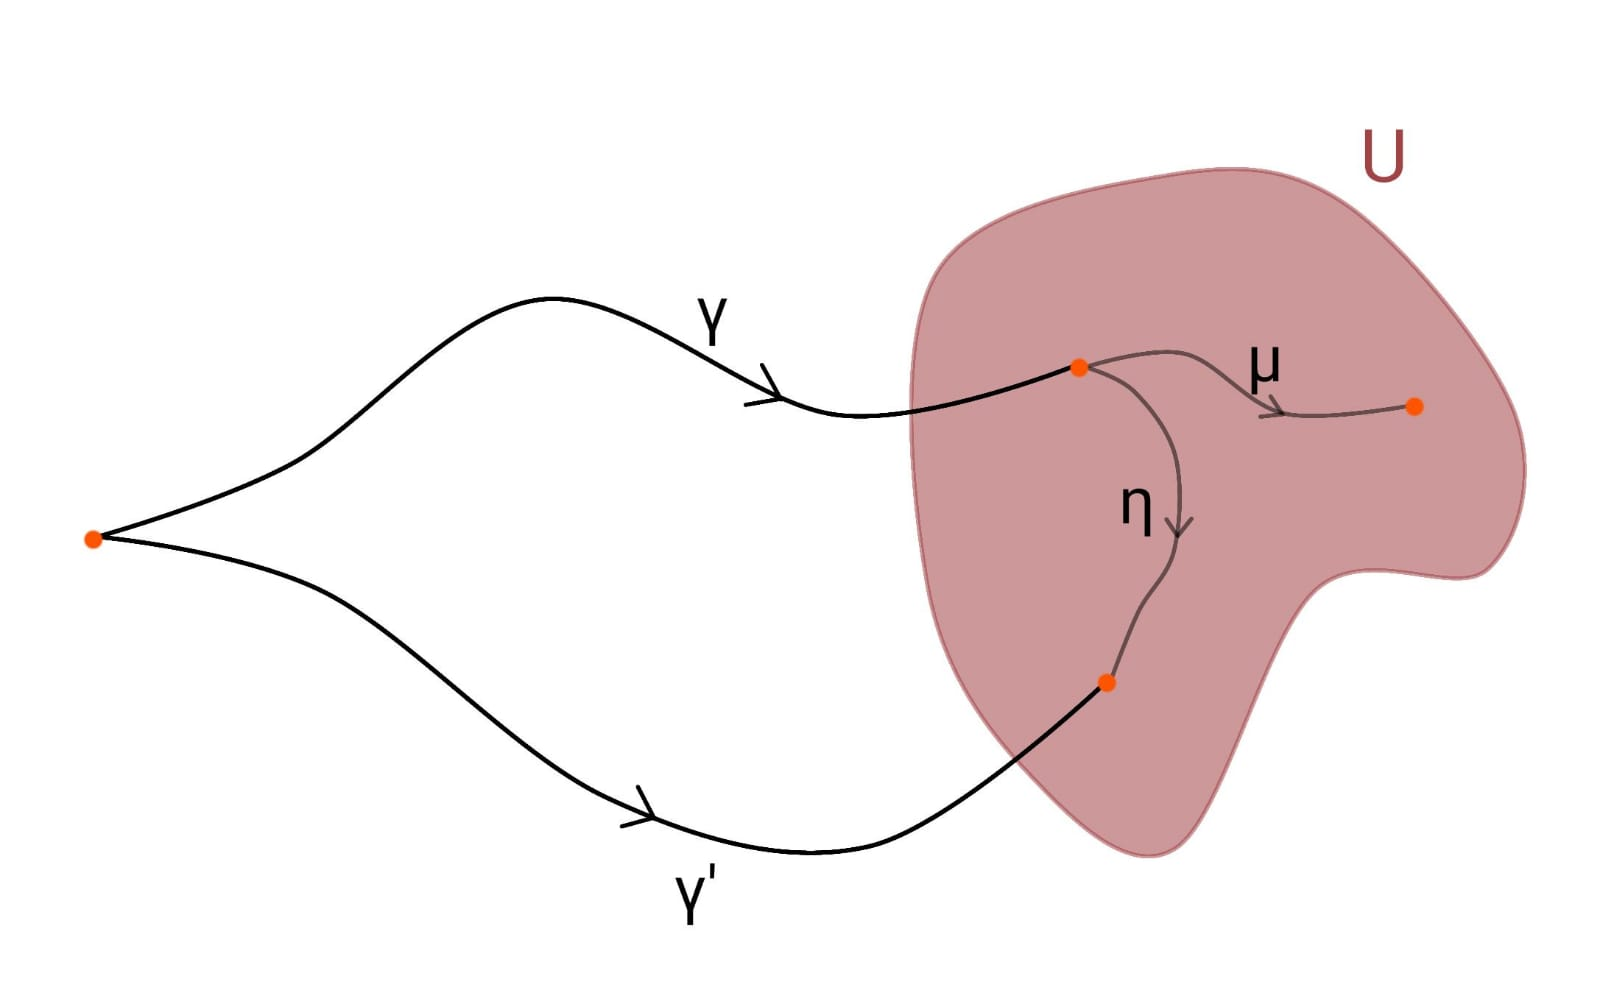
\includegraphics[width=0.8\linewidth]{conteudo/fig-cobertura-P(X,x_0).jpeg}
         \caption{Verificação de quando dois abertos $U_{[\gamma]}$ são iguais}
         \label{fig:cobertura-P(X,x_0)}
     \end{figure} 

     
     Verifiquemos que abertos desta forma constituem uma base para $P(X,x_0)$ e, além disso, que $q:U_{[\gamma]}\rightarrow U$ é um homeomorfismo, o que nos aproxima da verificação de que $q:P(X,x_0)\rightarrow X$ é um espaço de recobrimento.\newline

     De fato, temos as seguintes informações:

     \begin{enumerate}
        \item  $q:U_{[\gamma]}\rightarrow U$ é mapa injetor.\newline
        
        Escolhas diferentes de $\eta$ em $U$ que ligam $\gamma(1)$ a um mesmo ponto $x\in U$, isto é, dois caminhos $\eta_1$ e $\eta_2$ nessas condições tais que $q([\gamma*\eta_1])=q([\gamma*\eta_2])$, são tais que $\eta_1\sim \eta_2 (\text{rel }\partial I)$. Isso ocorre porque $i^*:\pi_1(U,x)\rightarrow \pi_1(X,x)$ é trivial, o que leva a conclusão de que dada a curva fechada $\eta_1* \overline{\eta_2}$ com ponto base $x$, temos a igualdade $[\eta_1* \overline{\eta_2}]=[c_x]\in \pi_1(X,x)$ e, portanto, $$\eta_1\sim\eta_1*(\overline{\eta_2}*\eta^2)\sim (\eta_1*\overline{\eta_2})*\eta^2\sim c_x*\eta_2\sim  \eta_2~(\text{rel }\partial I).$$  Dessa forma, $\gamma*\eta_1\sim \gamma*\eta_2 (\text{rel }\partial I)$ e, portanto, $[\gamma*\eta_1]=[\gamma*\eta_2]$. A situação é descrita na figura \ref{fig:restricao-de-q-é-injetor}.

        \begin{figure}[h!]
         \centering
         \includegraphics[width=0.8\linewidth]{conteudo/fig-restricao-de-q-é-injetor.jpeg}
         \caption{Restrição de $q$ a $U_{[\gamma]}$ é mapa injetor}
         \label{fig:restricao-de-q-é-injetor}
     \end{figure} 
     
         \item $q:U_{[\gamma]}\rightarrow U$ é mapa sobrejetor.\newline
         
         Como $U$ é conexo por caminhos, sempre é possível encontrar curva $\eta$ em $U$ que ligue $\gamma(1)$ a qualquer outro ponto de $U$.\newline
         
         \item $\tilde{\mathcal{B}}=\{U_{[\gamma]}|~U\in \mathcal{B}, \gamma:I\rightarrow X\text{ com }\gamma(0)=x_0\text{ e }\gamma(1)=x\in U\}$ é base para a topologia de $P(X,x_0)$.\newline
         
        Os abertos de $\tilde{\mathcal{B}}$ realmente cobrem $P(X,x_0)$ porque dado qualquer $[\gamma]\in P(X,x_0)$, se $\gamma(1)=x$, então existe $U\in \mathcal{B}$ vizinhança de $x$ de forma que $[\gamma]\in U_{[\gamma]}$.
        Além disso, dados $U_{[\gamma_1]} $ e $V_{\gamma_2}$ quaisquer em $\tilde{\mathcal{B}}$ e um elemento $[\gamma]\in U_{\gamma_1}\cap V_{\gamma_2}$, temos que $U_{[\gamma]}= U_{[\gamma_1]}$ e $V_{[\gamma]}=V_{[\gamma_2]}$, pois mostramos anteriormente que em geral $U_{[\gamma]}=U_{[\gamma']}$ se e somente se $[\gamma']\in U_{[\gamma]}$. Assim, $\gamma(1)\in U$, $\gamma(1)\in V$ e é possível tomar $W\in \mathcal{B}$ tal que $W\subset U\cap V$ é vizinhança de $\gamma(1)$, uma vez que $\mathcal{B}$ é base. Dessa forma, $W_{[\gamma]}\subset U_{[\gamma]}\cap V_{[\gamma]}=U_{[\gamma_1]}\cap V_{[\gamma_2]}$ pertence a $\tilde{\mathcal{B}}$ e contém $[\gamma]=[\gamma*c_{\gamma(1)}]$\newline
         

         \item $q:U_{[\gamma]}\rightarrow U$ é de fato homeomorfismo.\newline
         
            Seja $V\subset U$ aberto em $\mathcal{B}$. A pré-imagem desse aberto pela restrição de $q$ em $U_[\gamma]$ é $q^{-1}(V)\cap U_{[\gamma]}= V_{[\gamma']}$ para qualquer $[\gamma']\in U_{[\gamma]}$ tal que $\gamma'(1)\in V$, uma vez que $V_{[\gamma']} \subset U_{[\gamma']}=U_{[\gamma]}$ e já vimos que $q:V_{[\gamma']}\rightarrow V$ é uma bijeção. 
            
            De fato, se $V'\subset U$ é aberto qualquer, $V'=\underset{\lambda\in \Lambda, U_\lambda\in \mathcal{B}}{\bigcup} U_\lambda$ união enumerável de abertos e a pré imagem de $V'$ pela restrição de $q$ em $U_{[\gamma]}$ é $$q^{-1}(V')\cap U_{[\gamma]} =\underset{\lambda\in \Lambda, U_\lambda\in \mathcal{B}}{\bigcup} q^{-1}(U_\lambda)\cap U_{[\gamma]} = \underset{\lambda\in \Lambda, U_\lambda\in \mathcal{B}}{\bigcup} (U_\lambda)_{[\gamma_\lambda]}$$ para qualquer $[\gamma_\lambda]\in U_{[\gamma]}$ tal que $\gamma_\lambda(1)\in U_\lambda$. De fato, a pré-imagem é união enumerável de abertos e, portanto, aberta.
            
            
            Além disso, como $q(V_{[\gamma]})=V$ aberto e $\tilde{\mathcal{U}}$ é base, temos que dado qualquer aberto $V''\subset U_{[\gamma]}$ é $V''=\underset{\lambda \in \Lambda, U_\lambda \in \tilde{\mathcal{U}}}{\bigcup} U_\lambda$ união enumerável de abertos e então $q(V'')=\underset{\lambda \in \Lambda, U_\lambda \in \tilde{\mathcal{U}}}{\bigcup} q(U_\lambda)$, onde $q(U_\lambda)\in \mathcal{B}$ para todo $\lambda \in \Lambda$. Isto é, $q(V'')$ é união enumerável de abertos e, portanto, aberto.\newline

        \item $q:P(X,x_0)\rightarrow X$ é contínuo.\newline
        
            Para todo aberto $V\subset X$, temos que $V=\underset{\lambda\in \Lambda, V_\lambda \in \mathcal{B}}{\bigcup} V_\lambda$ para certos abertos $V_\lambda$ em $\mathcal{B}$.

            Temos que $$q^{-1}(V)=q^{-1}(\underset{\lambda\in \Lambda, V_\lambda \in \mathcal{B}}{\bigcup} V_\lambda)=\underset{\lambda\in \Lambda, V_\lambda \in \mathcal{B}}{\bigcup}q^{-1}(V_\lambda),$$ onde $q^{-1}(V_\lambda)=\underset{\gamma, (V_\lambda)_[\gamma] \in \tilde{\mathcal{B}}}{\bigcup} (V_\lambda)_{[\gamma]}$.

            Assim, todo $[\gamma]\in q^{-1}(V)$ é tal que $\gamma(1)\in V$ e, portanto, $\gamma(1)\in V_{\lambda_0}$ para algum $\lambda_0\in \Lambda$. Isto significa que $[\gamma]\in (V_{\lambda_0})_\gamma\subset q^{-1}(V)$ aberto. Portanto, $q^{-1}(V)$ é de fato aberto, como queríamos.\newline\newline
     \end{enumerate}


    Assim, temos que para todo $x\in X$ existe $U\in \mathcal{B}$ vizinhança de $x$ tal que  $p^{-1}(U)=\underset{[\gamma]}{\sqcup} U_{[\gamma]}$, onde cada $U_{[\gamma]}$ é homeomorfo a $U$. Essa união é disjunta pois se $U_{[\gamma_1]}\neq U_{[\gamma_2]}$ e $[\gamma]\in U_{[\gamma_1]}\cap U_{[\gamma_2]}$, então $U_{[\gamma]}=U_{[\gamma_1]}$ e $U_{[\gamma]}=U_{[\gamma_2]}$, o que implica $U_{[\gamma_1]}=U_{[\gamma_2]}$, uma contradição. Portanto, $U$ é aberto uniformemente recoberto de $X$ e isso conclui a nossa demonstração de que $P(X,x_0)$ é espaço de recobrimento.\newline

    Resta, por último, verificar que $P(X,x_0)$ é 1-conexo:

    \begin{enumerate}
        \item $P(X,x_0)$ é conexo por caminhos.\newline
        
            De fato, para todo $[\gamma]\in P(X,x_0)$, tome $\gamma_t:[0,1]\rightarrow X$ como a curva definida por 

            $$\begin{cases}
                \gamma(s), \text{ se }s\in [0,t]\\
                \gamma(t), \text{ se }s\in [t,1]
            \end{cases}$$

            Assim a curva $t\mapsto [\gamma_t]$ é um caminho em $P(X,x_0)$ que começa em $[c_{\gamma(0)}]=[c_{x_0}]$, curva constante em $\gamma(0)=x_0$, e termina em $[\gamma]$.

            Como isso vale para todo $[\gamma]$ em $P(X, x_0)$, então esse espaço é conexo por caminhos.\newline
        
        \item $\pi_1(P(X,x_0), [c_{x_0}])=0$\newline
        
            Para esta verificação mostraremos que $p_*: \pi_1(P(X,x_0), [c_{x_0}])\rightarrow \pi_1(X,x_0)$ é trivial.\newline

            Um elemento na imagem de $p_*$ é da forma $[\gamma]$ onde $\gamma$ é curva fechada com ponto base $x_0$ e seu levantamento também deve ser curva fechada, neste caso com ponto base $[c_{x_0}]$. Foi visto no item anterior que $t\mapsto [\gamma_t]$ levanta $\gamma$, começando em $[x_0]$ e terminando em $[\gamma_1]=[\gamma]$. Se esse levantamento é uma curva fechada, então $[\gamma]=[c_{x_0}]$ e o mapa de fato é trivial.

            Como $p_*$ é injetivo segundo o lema \ref{homomorfismo-induzido-por-recobrimento-prop}, então o fato de ser trivial implica $\pi_1(P(X,x_0), [c_{x_0}])=0$, como queríamos.\newline
        
    \end{enumerate}

    Assim, verificamos que $q: P(X,x_0)\rightarrow X$ é de fato um recobrimento 1-conexo e concluí-se por fim que, nas condições do enunciado, quando $X$ é semi-localmente simplesmente conexo, $X$ admite recobrimento 1-conexo.
    
\end{dem}

\begin{titlemize}{Lista de consequências}
	\item \hyperref[pertence-a-base-se-e-somente-se-possui-i-trivial]{Proposição - nova descrição da base $\mathcal{B}$};\\ %'consequencia1' é o label onde o conceito Consequência 1 aparece
    %\item \hyperref[espaço-1-conexo-def]{Espaço 1-conexo}
    \item \hyperref[recobrimento-universal]{Recobrimento universal}
\end{titlemize}

%---------------------------------------------------------------------------------------------------------------------!Draft!-----------------------------------------------------------------------------------------------------------------
\subsection{Descrição de $\tilde{\mathcal{B}}$ em termos de $X$} %afirmação aqui significa teorema/proposição/colorário/lema
\label{descrição-da-base-do-recobrimento-prop}
\begin{titlemize}{Lista de dependências}
	\item \hyperref[espaco-de-recobrimento-def]{Espaço de recobrimento};\\ %'dependencia1' é o label onde o conceito Dependência 1 aparece (--à arrumar um padrão para referencias e labels--) 
	\item \hyperref[espaço-1-conexo-def]{Espaço 1-conexo};\\
% quantas dependências forem necessárias.
\end{titlemize}


%Comentário sobre os objetos envolvidos na afirmação.



\begin{af}[Base para recobrimento 1-conexo]% ou af(afirmação)/prop(proposição)/corol(corolário)/lemma(lema)/outros ambientes devem ser definidos no preambulo de Alg.Top-Wiki.tex 
	Seja $p: E\rightarrow X$ um recobrimento com $X $ localmente conexo por caminhos e $E$ 1-conexo. A base $\tilde{\mathcal{B}}$ da topologia de $E$ definida em \ref{base-para-topologias-em-recobrimento-prop} pode ser descrita em termos de $X$ em dois casos:\newline

    \textbf{Caso 1:} Seja $U\in \mathcal{B}$ um aberto uniformemente recoberto com $x_0\in U$.\newline

    Em um espaço $\tilde{U}$ que seja placa de $U$ é possível levantar um caminho $\eta$ entre $x_0$ e $y_0$, em que $y_0\in U$ qualquer já que o espaço é conexo por caminhos, para um caminho $\tilde{\eta}$ entre $\tilde{x_0}$ e $\tilde{y_0}$ onde estes são pontos tais que $p(\tilde{x_0})=x_0$ e $p(\tilde{y_0})=y_0$.\newline

    Defina $U_{\tilde{x_0}}=\{\tilde{\eta}_{\tilde{x_0}}(1)|~\eta:I\rightarrow U\text{ e }\eta(0)=x_0\}$. A partir desta definição, é possível dizer que todas as placas de $U$ podem ser escritas como $U_{\tilde{x_0}}$ para algum $\tilde{x_0}$, que é o único valor existente na placa tal que $p(\tilde{x_0})=x_0$. Isto é,

    $$p^{-1}(U)=\underset{\tilde{x_0}\in p^{-1}(x_0)}{\sqcup} U_{\tilde{x_0}}$$
    


    \textbf{Caso 2:} Seja $U\subset X$ aberto conexo por caminhos e uniformemente recoberto, isto é, $U\in \mathcal{B}$. Tome $x\in U$ e seja $\tilde{x}\in E$ tal que $p(\tilde{x})=x$.\newline
    
    Fixe uma curva $\gamma: I\rightarrow X$ com $\gamma(0)=x_0$ e $\gamma(1)=x$, isto é, $[\gamma]\in q^{-1}(x)$. Note que $q$ é a função $q:P(X,x_0)\rightarrow X$ onde $P(X,x_0)=\{[\gamma]|~\gamma(0)=x_0\}$ definida por $q([\gamma])=\gamma(1)$.\newline
    
    Pode-se escrever $U$ como o espaço formado por $\gamma*\eta(1)$ para algum $\eta:I\rightarrow U$ tal que $\eta(0)=x$. Isto é, é possível descrever o aberto de $\tilde{\mathcal{B}}$ que é placa de $p$ sobre $U$ e vizinhança de $\tilde{x}$ como $$\tilde{U}_{\tilde{x}}=\{(\widetilde{\gamma*\eta})_{e_0}(1)|~\eta:I\rightarrow U,~\eta(0)=x\},$$ onde $e_0$ é tal que $\tilde{\gamma}_{e_0}(1)=\tilde{x}$.
    
    
    
	
\end{af}



\begin{titlemize}{Lista de consequências}
	\item \hyperref[pertence-a-base-se-e-somente-se-possui-i-trivial]{Proposição - nova descrição da base $\mathcal{B}$};\\ %'consequencia1' é o label onde o conceito Consequência 1 aparece
%	\item \hyperref[]{}
\end{titlemize}

%[Bianca]: Um arquivo tex pode ter mais de uma afirmação (ou definição, ou exemplo), mas nesse caso cada afirmação deve ter seu próprio label. Dar preferência para agrupar afirmações que dependam entre sí de maneira próxima (um teorema e seu corolário, por exemplo)
%---------------------------------------------------------------------------------------------------------------------!Draft!-----------------------------------------------------------------------------------------------------------------
\subsection{Base da topologia de $X$ possui $i^*$ trivial para todos os elementos quando há recobrimento 1-conexo} %afirmação aqui significa teorema/proposição/colorário/lema
\label{pertence-a-base-se-e-somente-se-possui-i-trivial}
\begin{titlemize}{Lista de dependências}
	\item \hyperref[base-para-topologias-em-recobrimento-prop]{Base para as topologias em um recobrimento};\\ %'dependencia1' é o label onde o conceito Dependência 1 aparece (--à arrumar um padrão para referencias e labels--) 
	\item \hyperref[recobrimento-1-conexo-prop]{Existe recobrimento 1-conexo se e somente se X slsc};\\
    \item \hyperref[descrição-da-base-do-recobrimento-prop]{Descrição de $\tilde{\mathcal{B}}$ em termos de $X$};\\
    \item \hyperref[1-conexo-prop]{Propriedades de 1-conexo};\\
    \item \hyperref[levantamento-de-homotopia-prop]{Levantamento de Homotopia}
% quantas dependências forem necessárias.
\end{titlemize}
%Comentário sobre os objetos envolvidos na afirmação.
\begin{prop}% ou af(afirmação)/prop(proposição)/corol(corolário)/lemma(lema)/outros ambientes devem ser definidos no preambulo de Alg.Top-Wiki.tex 
	Sejam $p:E\rightarrow X$ um recobrimento 1-conexo e $U\subset X$ um aberto conexo por caminhos. Então $U\in \mathcal{B}$, onde $\mathcal{B}$ é base para a topologia de $E$ conforme definida em \ref{base-para-topologias-em-recobrimento-prop}, se se somente se $i_*:\pi_1(U,x)\rightarrow \pi_1(X,x)$ é trivial.\\

\end{prop}
\begin{dem}
    Por um lado, se $U\in \mathcal{B}$ temos que, dada a inclusão $i:U\rightarrow X$, $i_*:\pi(U,x)\rightarrow \pi(X,x)$ é um mapa trivial segundo argumentação realizada no início da demonstração do Teorema \ref{recobrimento-1-conexo-prop}.\newline

    Por outro lado, se $i_*:\pi_1(U,x)\rightarrow \pi_1(X,x)$ é trivial, vamos verificar que $U$ é uniformemente recoberto. Em particular, verifiquemos que $p^{-1}(U)=\underset{[\gamma]\in q^{-1}(X)}{\bigsqcup} \tilde{U}_{[\gamma]}$ onde $$\tilde{U}_{[\gamma]}=\{(\widetilde{\gamma*\eta})_{\tilde{x}}(1)|~\eta:I\rightarrow U,~\eta(0)=x\}$$, da mesma forma que é descrito no "caso 2" da Afirmação \ref{descrição-da-base-do-recobrimento-prop}. Isto é, $\tilde{U}_{[\gamma]}\in \tilde{B}$.

    Para tal, verifiquemos:

    \begin{enumerate}
        \item $\tilde{U}_{[\gamma]}\subset p^{-1}(U)$ para todo $[\gamma]$ pois
        $$p(\tilde{U}_{[\gamma]})=\{p((\widetilde{\gamma*\eta})_{\tilde{x}}(1))|~\eta:I\rightarrow U,~\eta(0)=x\}=$$$$=\{(\gamma*\eta)(1)|~\eta:I\rightarrow U,~\eta(0)=x\}=\{\eta(1)\in U|~\eta:I\rightarrow U,~\eta(0)=x\}\subset U$$\newline

        \item $p^{-1}(U)\subset \underset{[\gamma]\in q^{-1}(x)}{\bigcup} \tilde{U}_{[\gamma]}$

        Seja $\tilde{y}\in p^{-1}(U)$, seja $\eta:I\rightarrow U$ com $\eta(0)=x$ e $\eta(1)=y=p(\tilde{y})$ e seja $\tilde{x}=\tilde{\overline{\eta}}_{\tilde{y}}(1)$, de forma que $p(\tilde{x})=x$.

        Seja $ \xi:I\rightarrow E$ com $\xi(0)=e_0$, $\xi(1)=\tilde{x}$ e seja $\gamma=p\circ \xi$. Então $ \tilde{y}\in \tilde{U}_{[\gamma]}$ pois $(\widetilde{\gamma * \eta})_{e_0}(1)=\tilde{\eta}_{\tilde{x}}(1)=\tilde{y}$.\newline

        \item Se $[\gamma_0]\neq [\gamma_1]\in q^{-1}(x)$, então $ \tilde{U}_{[\gamma_0]}\cap \tilde{U}_{[\gamma_1]}=\emptyset$

        Suponha que $\tilde{y}\in \tilde{U}_{[\gamma_0]}\cap\tilde{U}_{[\gamma_1]}$. Sejam $\eta_0, \eta_1: I\rightarrow U$ curvas tais que $(\widetilde{\gamma_0*\eta_0})_{e_0}(1)=(\widetilde{\gamma_1*\eta_1})_{e_0}(1)=\tilde{y}$, como representado na figura \ref{fig:classes-distintas-de-curvas} a seguir.

\begin{figure}[h!]
         \centering
         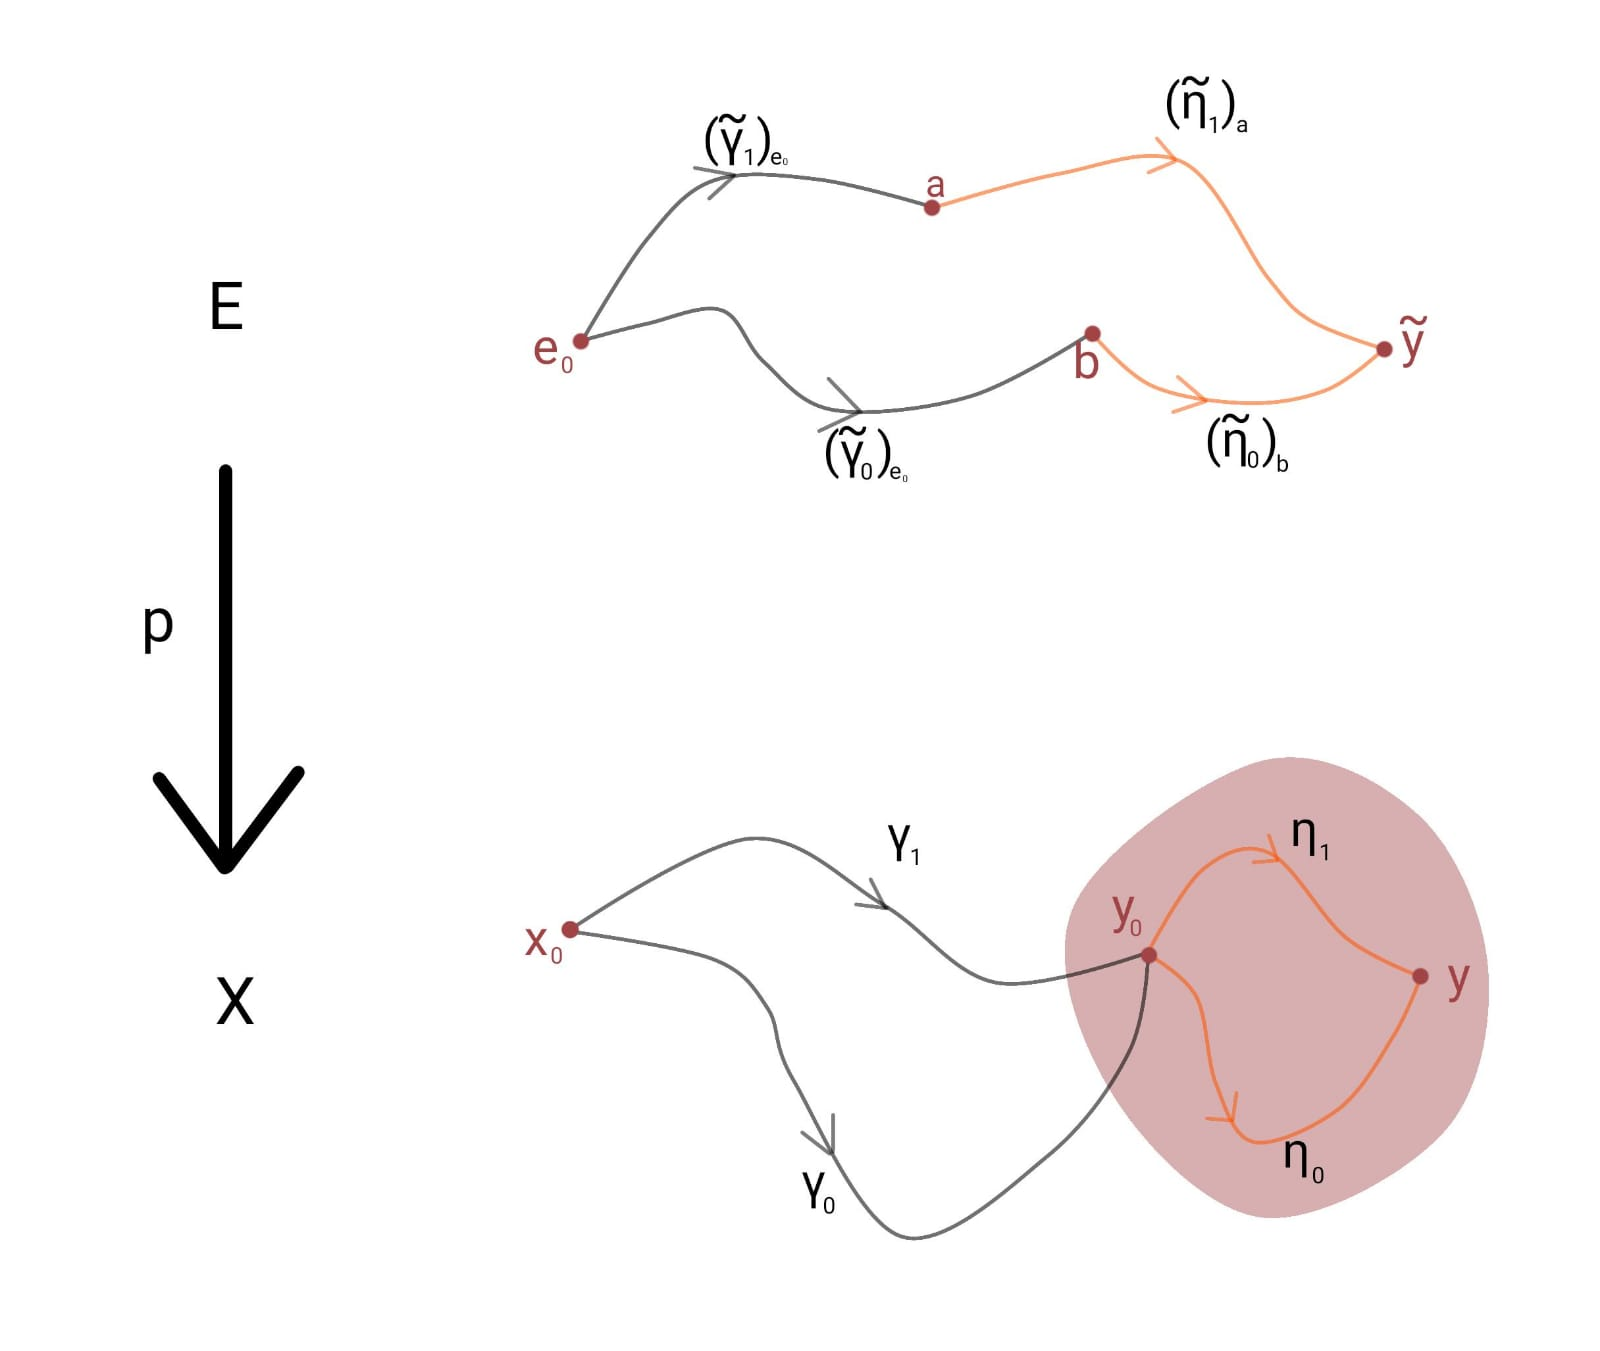
\includegraphics[width=0.8\linewidth]{conteudo/fig-classes-distintas-de-curvas.jpeg}
         \caption{Classes distintas de curvas, mas $\tilde{y}$ na intersecção dos abertos}
         \label{fig:classes-distintas-de-curvas}
     \end{figure} 

        
        Assim, temos que $p\circ(\widetilde{\gamma_0*\eta_0})_{e_0}(1)=y=p\circ(\widetilde{\gamma_1*\eta_1})_{e_0}(1)$ e portanto $\eta_0(1)=y=\eta_1(1)$.

        Na mesma figura, é possível notar que $\eta_0*\overline{\eta}_1$ é um laço em $U$ com ponto base $y$. Como nos foi dado que $i^*:\pi(U,x)\rightarrow \pi_1(X,x)$ é trivial e $U$ conexo por caminhos, temos que

        $$(\eta_0*\overline{\eta}_1)\sim c_y~(\text{rel}~\partial I) \Rightarrow (\widetilde{\eta_0 * \overline{\eta_1}})_{\tilde{y}}\sim  c_{\tilde{y}}~(\text{rel}~\partial I)\Rightarrow (\tilde{\gamma}_0)_{e_0}(1)=(\tilde{\gamma}_1)_{e_0}(1),$$ diferentemente do que a imagem indica.

        Como $E$ é 1-conexo, utilizando a Proposição \ref{1-conexo-prop} concluí-se que $[\gamma_0]=[\gamma_1]$, um absurdo por contradizer a hipótese inicial.\newline
        

    
        \item A restrição $p|_{\tilde{U}_{[\gamma]}}:\tilde{U}_{[\gamma]}\rightarrow U $ é bijeção

        Para verificar a sobrejetividade basta notar que para todo $y\in U$ é possível tomar a curva $\eta:I\rightarrow U$ tal que $\eta(0)=x$ e $\eta(1)=y$. Temos que se $\tilde{y}=(\widetilde{\gamma*\eta})_{e_0}(1)\in \tilde{U}_{[\gamma]}$, então $p(\tilde{y})=y$, como queríamos.

        Para a verificação da injetividade, basta supor que $p((\widetilde{\gamma*\eta_0})_{e_0}(1))=p((\widetilde{\gamma*\eta_1})_{e_0}(1))$ onde $\eta_0, \eta_1:I\rightarrow U$ são tais que $\eta_0(0)=x=\eta_1(0)$ e $\eta_0(1)=\eta_1(1)$. Portanto, $\eta_0*\overline{\eta}_1$ é laço e assim $\eta_0\sim \eta_1~(\text{rel }\partial I)$.
        Isso significa que, se $\tilde{x}=\tilde{\gamma}_{e_0}(1)$, então $(\tilde{\eta}_0)_{\tilde{x}}(1)= (\tilde{\eta}_1)_{\tilde{x}}(1)$ segundo Corolário presente em \ref{levantamento-de-homotopia-prop}. Assim, $(\widetilde{\gamma*\eta_0})_{e_0}(1)=(\gamma*\eta_1)_{e_0}(1)$.\newline

        \item A restrição $p|_{\tilde{U}_{[\gamma]}}$ é aplicação aberta pois $\tilde{U}_{[\gamma]}\in \tilde{\mathcal{B}}$ é uma placa do recobrimento.\newline
    \end{enumerate}

    Assim, verificamos que $U$ é uniformemente recoberto, isto é, $U \in \mathcal{B}$ como queríamos.\newline
\end{dem}

O resultado acima implica que a base $\mathcal{B}$ pode ser descrita como $\mathcal{B}=\{U\subset X|~U\text{ é conexo por caminhos e }i_*:\pi_1(U,x)\rightarrow \pi_1(X,x)\text{ é trivial}\}$

%\begin{titlemize}{Lista de consequências}
%	\item \hyperref[consequencia1]{Consequência 1};\\ %'consequencia1' é o label onde o conceito Consequência 1 aparece
%	\item \hyperref[]{}
%\end{titlemize}

%[Bianca]: Um arquivo tex pode ter mais de uma afirmação (ou definição, ou exemplo), mas nesse caso cada afirmação deve ter seu próprio label. Dar preferência para agrupar afirmações que dependam entre sí de maneira próxima (um teorema e seu corolário, por exemplo)

%%% Local Variables:
%%% mode: LaTeX
%%% TeX-master: "../Alg.Top-Wiki"
%%% End:

\end{document}


%novos assuntos/secções devem ser adicionados através do comando \import{conteudo/}{assunto} para adicionar o arquivo conteudo/assunto.tex

%%% Local Variables:
%%% mode: LaTeX
%%% TeX-master: t
%%% End:
